\section{Seconda parte}
\subsection{Introduzione}
Come step successivo si è deciso di modificare il criterio di early stopping dei modelli inserendo come variabile anche le emissioni.
Il classico criterio di early stopping prevede di fermare l'addestramento del modello quando lo score ottenuto con il validation set non migliora per un certo numero di epoche consecutive.


\begin{figure}[H]
    \centering
    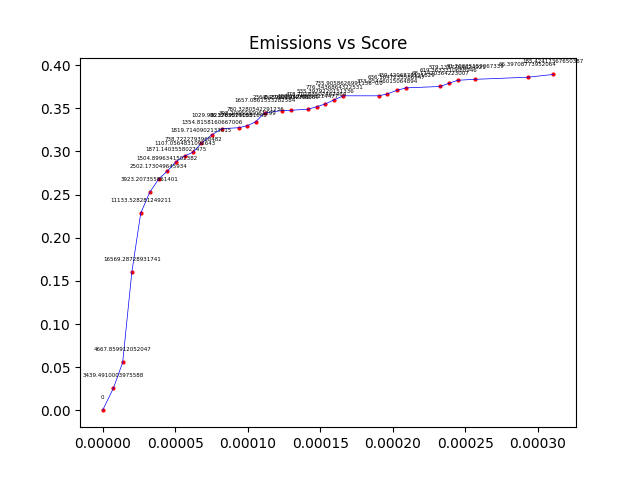
\includegraphics[scale=1]{images/curve_emissions_score.png}
    \caption{Andamento dello score in funzione delle emissioni}
\end{figure}

\noindent Questa curva mostra mostra il comportamento dello score in funzione delle emissioni. In particolare si tiene traccia solo delle epoche in cui lo score è migliorato rispetto al risultato migliore.
Si può notare come la curva presenti una forte crescita iniziale, per poi stabilizzarsi e avere un andamento quasi lineare.
Questo andamento lineare indica dunque un miglioramento molto piccolo dello score rispetto alle emissioni.

\noindent Il criterio di early stopping con emissioni si pone dunque come obiettivo quello di fermare l'addestramento del modello quando il miglioramento dello score rispetto alle emissioni è troppo piccolo.
L'idea alla base sarebbe quello di fermare l'addestramento studiando la derivata della curva. Siccome i valori sono discreti, si è deciso di approssimare la derivata con la differenza tra due punti consecutivi \footnote{Metodo delle differenze divise di ordine 1}{} mediante la seguente formula:
\begin{equation}
    \frac{f(x_{i+1}) - f(x_i)}{x_{i+1} - x_i}
\end{equation}

\noindent Quando la differenza tra due rapporti consecutivi è minore di una certa soglia, per un certo numero di volte consecutive, si ferma l'addestramento del modello.

\subsection{Parte esplorativa}
\subsubsection{Primo esperimento}

Il primo esperimento è stato compiuto con il dataset MovieLens-1m. La soglia è stata impostata a 50 e il numero di epoche consecutive a 5.

\begin{table}[H]
    \centering
    \footnotesize
    \setlength\tabcolsep{0pt}
    \begin{tabularx}{\textwidth}{|X|X|}
        \hline
        \textbf{Criterio classico} & \textbf{Criterio modificato} \\
        \hline
        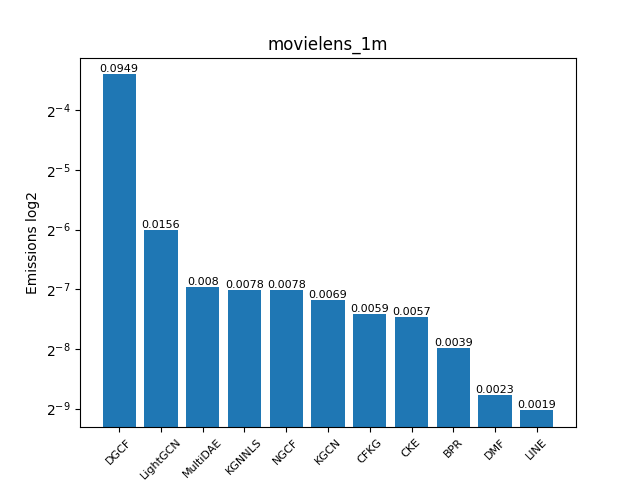
\includegraphics[width=\linewidth, trim=0 0 0 0]{images/emissions_movielens_1m_earlyClassic.png} &
        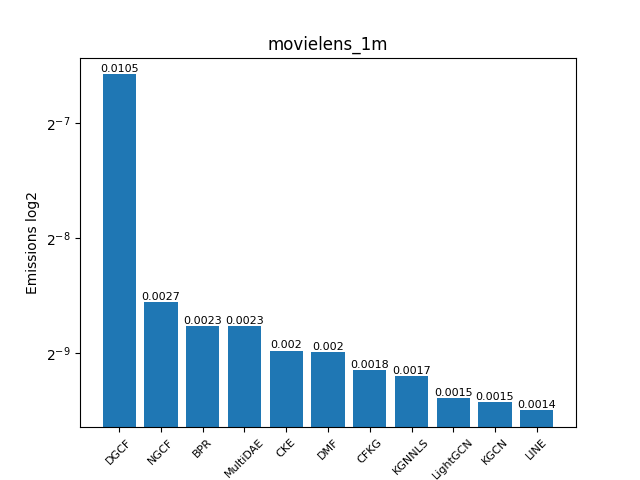
\includegraphics[width=\linewidth, trim=0 0 0 0]{images/emissions_movielens_1m_earlyModified.png} \\
        \hline
    \end{tabularx}
    \caption{Emissioni con criterio classico e modificato}
    \label{tab:emissions_info}
\end{table}

\noindent Si può dunque chiaramente notare come usando il nuovi criterio di early stopping le emissioni siano molto più basse rispetto al criterio classico.

\begin{table}[H]
    \centering
    \resizebox{\textwidth}{!}{
    \begin{tabular}{|c|c|c|c|}
        \hline
        \textbf{Modello} & \textbf{Emissioni criterio classico (g)} & \textbf{Emissioni criterio nuovo (g)} & \textbf{\% riduzione emissioni}\\
        \hline
        BPR & 3.9484 & 2.3033 & 41.6647 \\
        \hline
        CKFG & 5.881 & 1.767 & 69.9418 \\
        \hline
        CKE & 5.68394 & 1.9837 & 65.09955 \\
        \hline
        DMF & 2.2927 & 1.9667 & 14.2158 \\
        \hline
        KGCN & 6.8754 & 1.454 & 78.8522 \\
        \hline
        KGNNLS & 7.763 & 1.70177 & 78.0785 \\
        \hline
        LINE & 1.9128 & 1.3831 & 27.6935 \\
        \hline
        MultiDAE & 8.0303 & 2.29608 & 71.40737 \\
        \hline
        LightGCN & 15.626 & 1.4926 & 90.4481 \\
        \hline
        NGCF & 7.7582 & 2.6601 & 65.7126 \\
        \hline
        DGCF & 94.903 & 10.4625 & 88.9756\\
        \hline
    \end{tabular}
    }
    \caption{Confronto delle emissioni}
\end{table}

\noindent Si può dunque notare come in generale la percentuale di riduzione delle emissioni è molto alta



\begin{figure}[H]
    \centering
    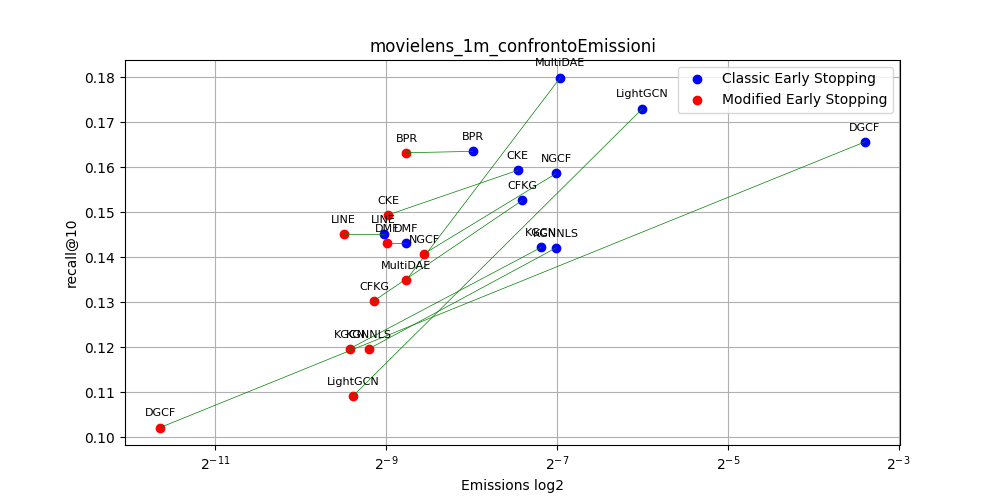
\includegraphics[width=\linewidth, trim=0 0 0 0]{images/recall@10_movielens_1m_comparison.png}
    \caption{Confronto score recall@10 con dataset MovieLens-1m}
    
\end{figure}

\begin{figure}[H]
    \centering
    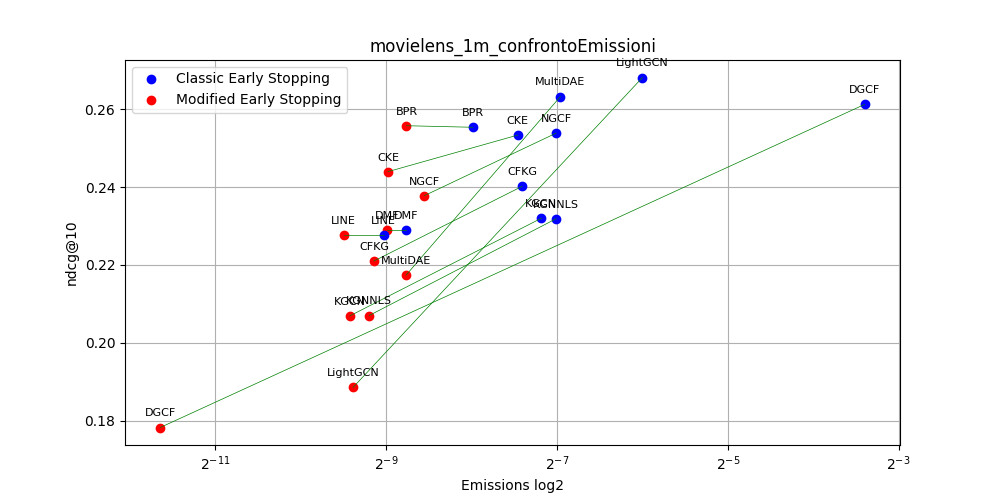
\includegraphics[width=\linewidth, trim=0 0 0 0]{images/ndcg@10_movielens_1m_comparison.png}
    \caption{Confronto score ndcg@10 con dataset MovieLens-1m}
    
\end{figure}

\begin{figure}[H]
    \centering
    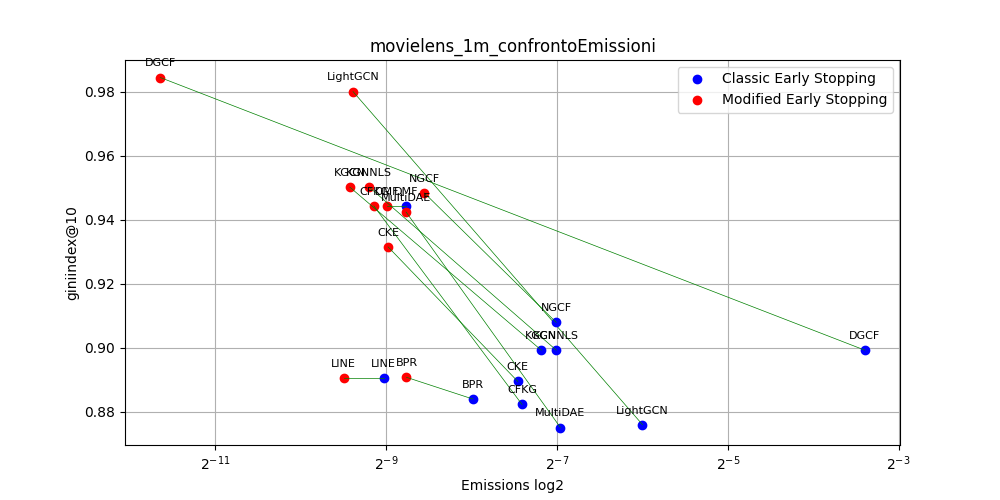
\includegraphics[width=\linewidth, trim=0 0 0 0]{images/giniindex@10_movielens_1m_comparison.png}
    \caption{Confronto score giniindex@10 con dataset MovieLens-1m}
\end{figure}

\begin{figure}[H]
    \centering
    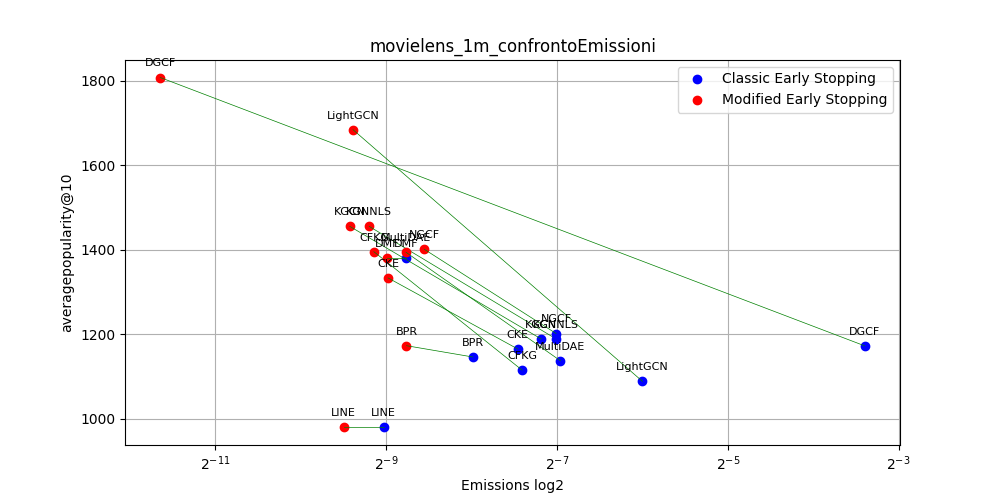
\includegraphics[width=\linewidth, trim=0 0 0 0]{images/averagepopularity@10_movielens_1m_comparison.png}
    \caption{Confronto score averagepopularity@10 con dataset MovieLens-1m}
\end{figure}




\begin{table}[H]
    \centering
    \resizebox{\textwidth}{!}{
        \begin{tabular}{|c|c|c|c|c|}
            \hline
            \textbf{Modello} & \textbf{Metrica} & \textbf{Score criterio classico} & \textbf{Score criterio nuovo} & \textbf{\% riduzione score}\\
            \hline
            BPR & recall@10 & 0.1635 & 0.1632 & 0.1835\\
            \hline
            CFKG & recall@10 & 0.1526 & 0.1303 & 14.6134\\
            \hline
            CKE & recall@10 & 0.1593 & 0.1494 & 6.2147\\
            \hline
            DMF & recall@10 & 0.1432 & 0.1432 & 0.0\\
            \hline
            KGCN & recall@10 & 0.1422 & 0.1197 & 15.8228\\
            \hline
            KGNNLS & recall@10 & 0.1421 & 0.1197 & 15.7635\\
            \hline
            LINE & recall@10 & 0.1451 & 0.1451 & 0.0\\
            \hline
            MultiDAE & recall@10 & 0.1799 & 0.1349 & 25.0139\\
            \hline
            LightGCN & recall@10 & 0.173 & 0.1092 & 36.8786\\
            \hline
            NGCF & recall@10 & 0.1586 & 0.1408 & 11.2232\\
            \hline
            DGCF & recall@10 & 0.1656 & 0.1022 & 38.2850\\
            \hline
            BPR & ndcg@10 & 0.2554 & 0.2558 & -0.1566\\
            \hline
            CFKG & ndcg@10 & 0.2402 & 0.221 & 7.9933\\
            \hline
            CKE & ndcg@10 & 0.2534 & 0.244 & 3.7096\\
            \hline
            DMF & ndcg@10 & 0.2289 & 0.2289 & 0.0\\
            \hline
            KGCN & ndcg@10 & 0.232 & 0.2069 & 10.819\\
            \hline
            KGNNLS & ndcg@10 & 0.2319 & 0.207 & 10.737\\
            \hline
            LINE & ndcg@10 & 0.2277 & 0.2277 & 0.0\\
            \hline
            MultiDAE & ndcg@10 & 0.2633 & 0.2174 & 17.433\\
            \hline
            LightGCN & ndcg@10 & 0.2682 & 0.1885 & 29.717\\
            \hline
            NGCF & ndcg@10 & 0.2539 & 0.2378 & 6.3411\\
            \hline
            DGCF & ndcg@10 & 0.2613 & 0.1782 & 31.8025\\
            \hline
            BPR & averagepopularity@10 & 1146.3572 & 1173.1199 & -2.3346\\
            \hline
            CFKG & averagepopularity@10 & 1115.4498 & 1395.6098 & -25.1163\\
            \hline
            CKE & averagepopularity@10 & 1165.2413 & 1333.5153 & -14.4411\\
            \hline
            DMF & averagepopularity@10 & 1379.7292 & 1379.7292 & 0.0\\
            \hline
            KGCN & averagepopularity@10 & 1188.9582 & 1455.5651 & -22.4236\\
            \hline
            KGNNLS & averagepopularity@10 & 1188.8981 & 1455.58 & -22.4310\\
            \hline
            LINE & averagepopularity@10 & 979.498 & 979.498 & 0.0\\
            \hline
            MultiDAE & averagepopularity@10 & 1137.4597 & 1394.0944 & -22.5621\\
            \hline
            LightGCN & averagepopularity@10 & 1088.741 & 1684.4149 & -54.7122\\
            \hline
            NGCF & averagepopularity@10 & 1201.8831 & 1401.4325 & -16.6031\\
            \hline
            DGCF & averagepopularity@10 & 1172.6874 & 1807.9828 & -54.1743\\
            \hline
            BPR & giniindex@10 & 0.8839 & 0.8907 & -0.7693\\
            \hline
            CFKG & giniindex@10 & 0.8822 & 0.9443 & -7.0392\\
            \hline
            CKE & giniindex@10 & 0.8894 & 0.9315 & -4.7335\\
            \hline
            DMF & giniindex@10 & 0.9443 & 0.9443 & 0.0\\
            \hline
            KGCN & giniindex@10 & 0.8992 & 0.9502 & -5.6717\\
            \hline
            KGNNLS & giniindex@10 & 0.8992 & 0.9502 & -5.6717\\
            \hline
            LINE & giniindex@10 & 0.8904 & 0.8904 & 0.0\\
            \hline
            MultiDAE & giniindex@10 & 0.875 & 0.9424 & -7.7029\\
            \hline
            LightGCN & giniindex@10 & 0.8759 & 0.9801 & -11.8963\\
            \hline
            NGCF & giniindex@10 & 0.9079 & 0.9484 & -4.4608\\
            \hline
            DGCF & giniindex@10 & 0.8992 & 0.9845 & -9.4862\\
            \hline
        \end{tabular}
    }
    \caption{Confronto degli score tra criteri e modelli}
\end{table}

\begin{figure}[H]
    \centering
    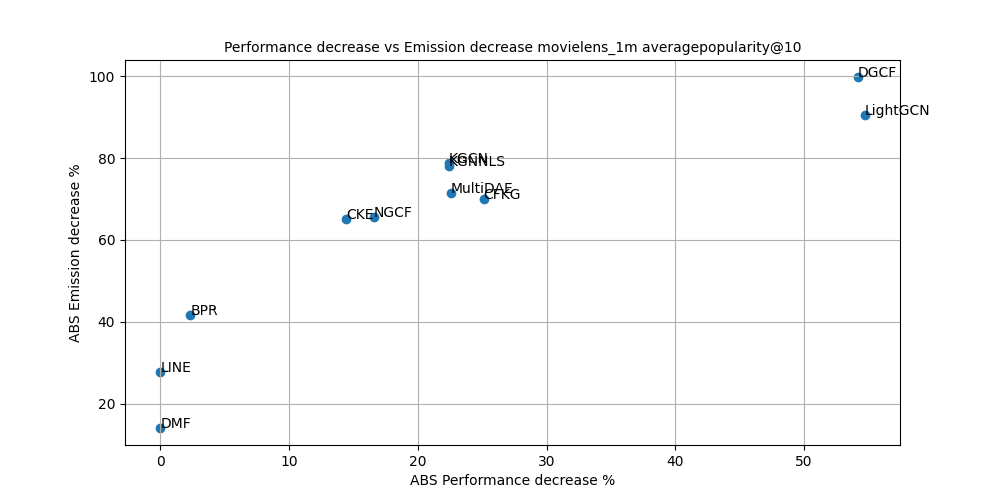
\includegraphics[scale=0.5]{images/decrement_averagepopularity@10_movielens_1m.png}
    \caption{Decremento di averagepopularity@10}
\end{figure}

\begin{figure}[H]
    \centering
    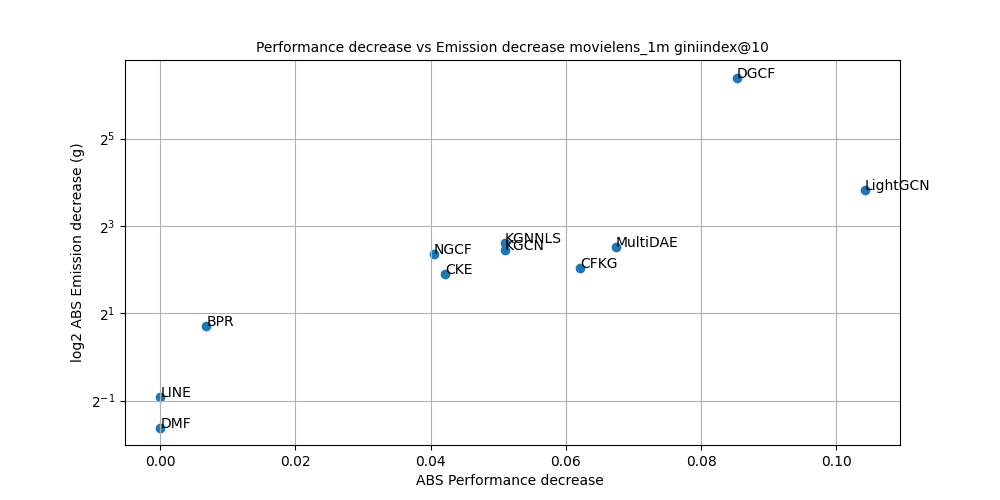
\includegraphics[scale=0.5]{images/decrement_giniindex@10_movielens_1m.png}
    \caption{Decremento di giniindex@10}
\end{figure}

\begin{figure}[H]
    \centering
    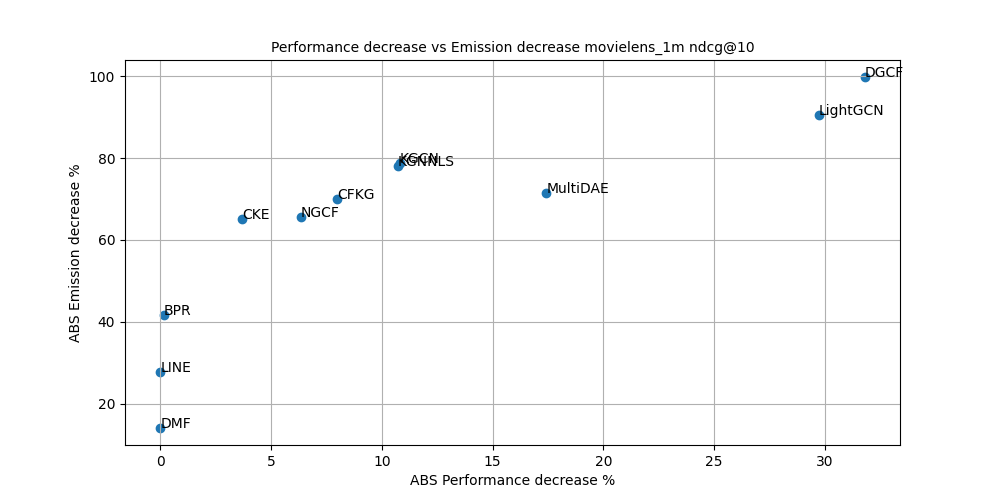
\includegraphics[scale=0.5]{images/decrement_ndcg@10_movielens_1m.png}
    \caption{Decremento di ndcg@10}
\end{figure}

\begin{figure}[H]
    \centering
    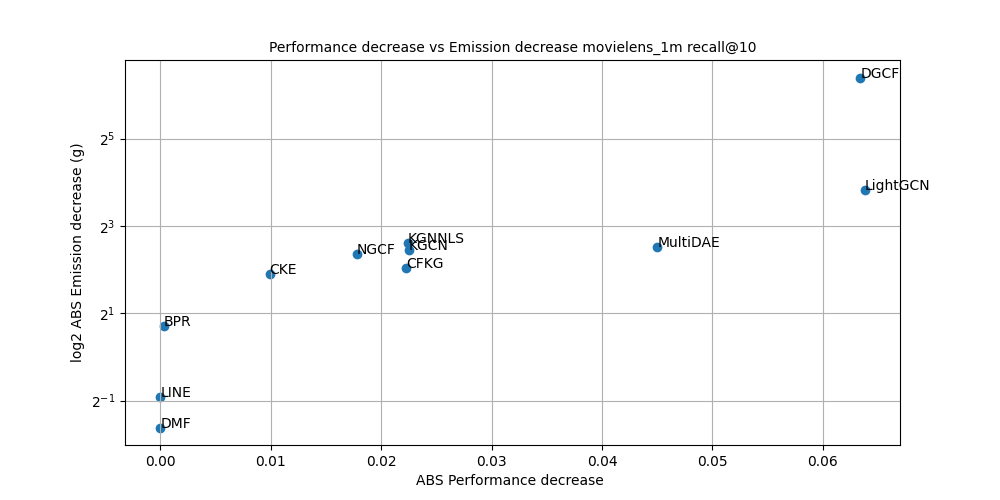
\includegraphics[scale=0.5]{images/decrement_recall@10_movielens_1m.png}
    \caption{Decremento di recall@10}
\end{figure}


\noindent Per quanto riguarda giniindex e averagepopularity un punteggio più basso è migliore, mentre per recall e ndcg un punteggio più alto è migliore.
Ecco perchè la percentuale di riduzione degli score è negativa per giniindex e averagepopularity.

\noindent Confrontando le percentuali di riduzione delle emissioni e degli score si può notare la riduzione delle emissioni è molto più alta rispetto alla riduzione degli score.

\noindent BPR tende a mantenere le stesse perfomance con entrambi i criteri a fronte di emissioni molto più basse.
Possiamo notare come LINE e DMF non abbiano subito variazioni di score, mentre LightGCN e DGCF abbiano subito una riduzione molto alta (in percentuale comunque molto inferiore rispetto alla riduzione delle emissioni).
Probabilmente per LINE e DMF il criterio di early stopping classico ha portato ad eseguire qualche epoca in più ma che non ha portato a miglioramenti.

\subsubsection{Secondo esperimento}
Il secondo esperimento è stato compiuto con il dataset LFM-1b\_artist\_20U50I\_25strat. La soglia è stata impostata a 30 e il numero di epoche consecutive a 7, dunque un criterio più stringente (una differenza tra i rapporti consecutivi minore da verificare per più miglioramenti consecutivi).


\begin{table}[H]
    \centering
    \footnotesize
    \setlength\tabcolsep{0pt}
    \begin{tabularx}{\textwidth}{|X|X|}
        \hline
        \textbf{Criterio classico} & \textbf{Criterio modificato} \\
        \hline
        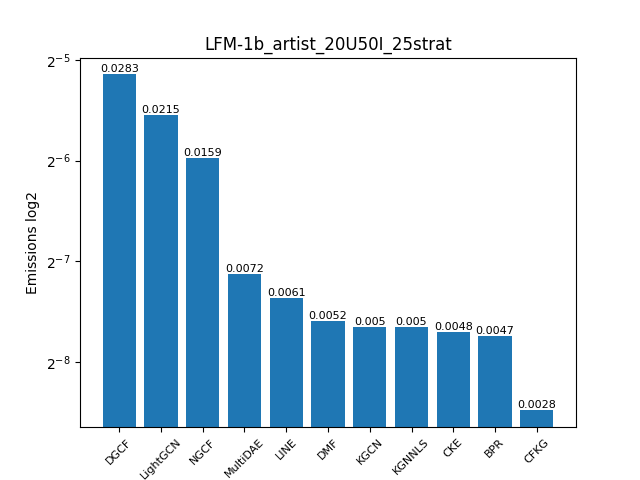
\includegraphics[width=\linewidth, trim=0 0 0 0]{images/emissions_LFM-1b_artist_20U50I_25strat_earlyClassic.png} &
        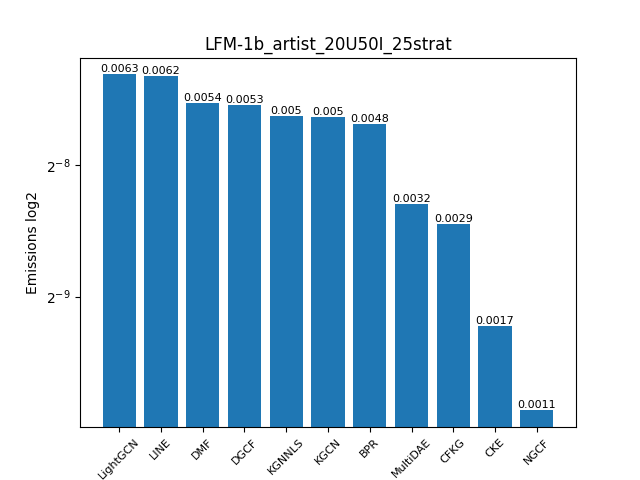
\includegraphics[width=\linewidth, trim=0 0 0 0]{images/emissions_LFM-1b_artist_20U50I_25strat_earlyModified.png} \\
        \hline
    \end{tabularx}
    \caption{Emissioni con criterio classico e modificato}
    \label{tab:emissions_info}
\end{table}



\begin{table}[H]
    \centering
    \resizebox{\textwidth}{!}{
    \begin{tabular}{|c|c|c|c|}
        \hline
        \textbf{Modello} & \textbf{Emissioni criterio classico (g)} & \textbf{Emissioni criterio nuovo (g)} & \textbf{\% riduzione emissioni}\\
        \hline
        BPR & 4.6785 & 4.8381 & -3.4125 \\
        \hline
        CKFG & 2.8024 & 2.8539 & -1.8368 \\
        \hline
        CKE & 4.8062 & 1.6694 & 65.2659 \\
        \hline
        DMF & 5.1886 & 5.3978 & -4.0321 \\
        \hline
        KGCN & 4.9718 & 5.0108 & -0.7863 \\
        \hline
        KGNNLS & 4.9701 & 5.0453 & -1.5133 \\
        \hline
        LINE & 6.0602 & 6.2294 & -2.7912 \\
        \hline
        MultiDAE & 7.1668 & 3.1731 & 55.7245 \\
        \hline
        LightGCN & 21.4561 & 6.2812 & 70.7256 \\
        \hline
        NGCF & 15.8887 & 1.0731 & 93.2463 \\
        \hline
        DGCF & 28.2945 & 5.3468 & 81.103\\
        \hline
    \end{tabular}
    }
    \caption{Confronto delle emissioni}
\end{table}

\noindent Il criterio più stringente mostra chiaramente come la riduzione delle emissioni sia meno alta rispetto al primo esperimento.
Per alcuni modelli vengono registrate addirittura delle variazioni negative, ovvero le emissioni sono aumentate rispetto al criterio classico. Questo potrebbe dipende da un picco di consumi dell'hardware in un certo momento, dovuto magari a qualche processo in background.
NGCF è l'unico modello in cui si registra un'aumento della percentuale di riduzione delle emissioni rispetto al primo esperimento.


\begin{figure}[H]
    \centering
    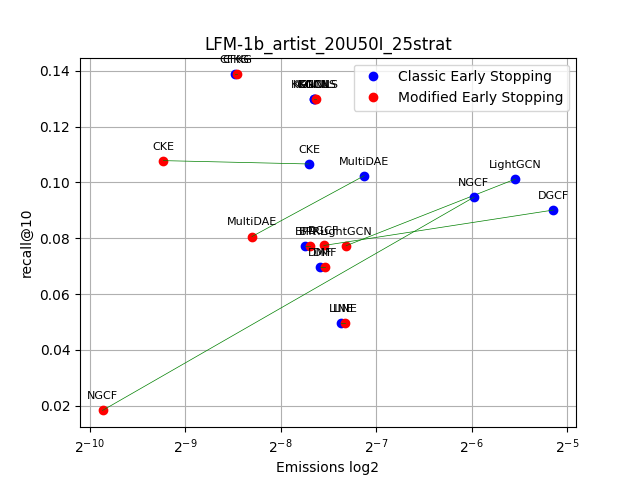
\includegraphics[width=\linewidth, trim=0 0 0 0]{images/recall@10_LFM-1b_artist_20U50I_25strat_comparison.png}
    \caption{Confronto score recall@10 con dataset LFM-1b\_artist\_20U50I\_25strat}
    
\end{figure}

\begin{figure}[H]
    \centering
    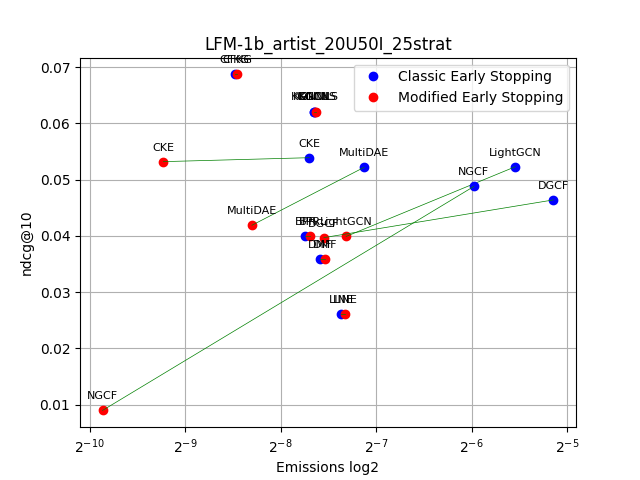
\includegraphics[width=\linewidth, trim=0 0 0 0]{images/ndcg@10_LFM-1b_artist_20U50I_25strat_comparison.png}
    \caption{Confronto score ndcg@10 con dataset LFM-1b\_artist\_20U50I\_25strat}
    
\end{figure}

\begin{figure}[H]
    \centering
    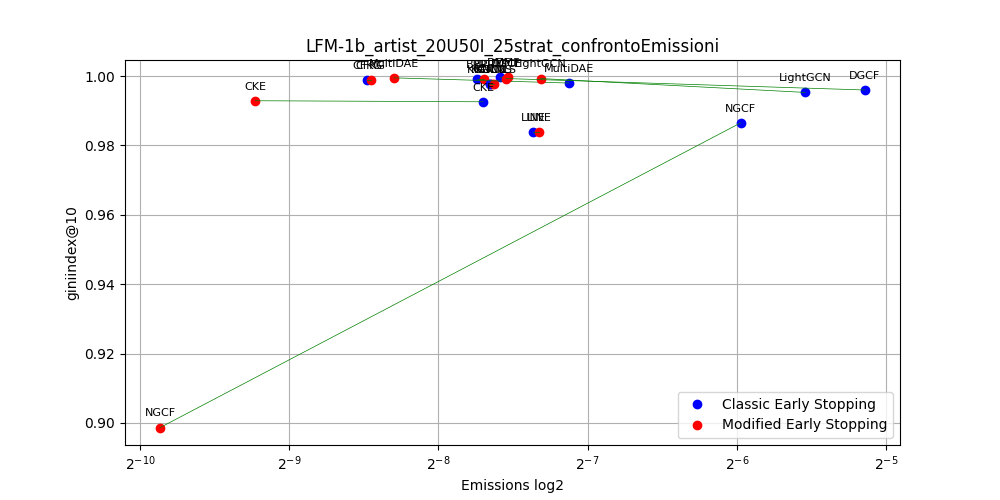
\includegraphics[width=\linewidth, trim=0 0 0 0]{images/giniindex@10_LFM-1b_artist_20U50I_25strat_comparison.png}
    \caption{Confronto score giniindex@10 con dataset LFM-1b\_artist\_20U50I\_25strat}
\end{figure}

\begin{figure}[H]
    \centering
    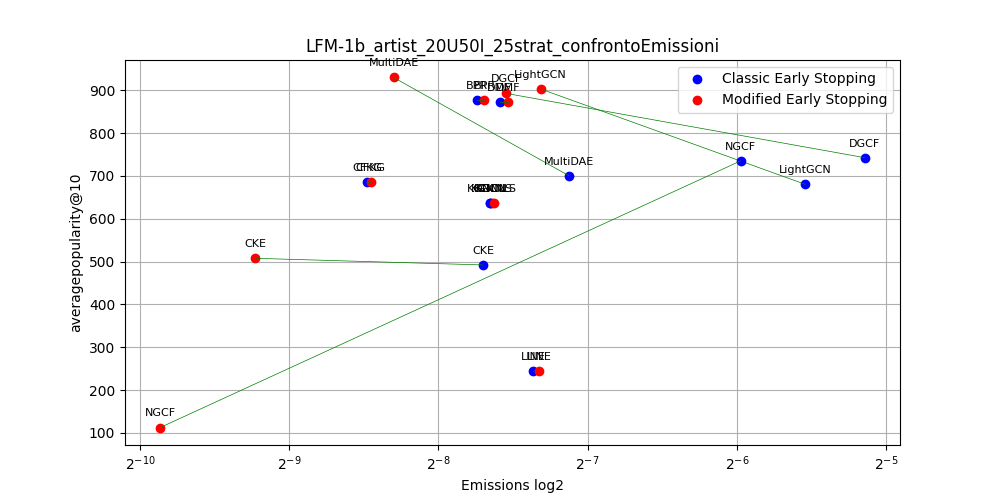
\includegraphics[width=\linewidth, trim=0 0 0 0]{images/averagepopularity@10_LFM-1b_artist_20U50I_25strat_comparison.png}
    \caption{Confronto score averagepopularity@10 con dataset LFM-1b\_artist\_20U50I\_25strat}
\end{figure}


\begin{table}[H]
    \centering
    \resizebox{\textwidth}{!}{
        \begin{tabular}{|c|c|c|c|c|}
            \hline
            \textbf{Modello} & \textbf{Metrica} & \textbf{Score criterio classico} & \textbf{Score criterio nuovo} & \textbf{\% riduzione score}\\
            \hline
            BPR              & recall@10         & 0.0772                            & 0.0772                         & 0.0                         \\ \hline
            CFKG             & recall@10         & 0.1387                            & 0.1387                         & 0.0                         \\ \hline
            CKE              & recall@10         & 0.1066                            & 0.1078                         & -1.1257                     \\ \hline
            DMF              & recall@10         & 0.0698                            & 0.0698                         & 0.0                         \\ \hline
            KGCN             & recall@10         & 0.1299                            & 0.1299                         & 0.0                         \\ \hline
            KGNNLS           & recall@10         & 0.1299                            & 0.1299                         & 0.0                         \\ \hline
            LINE             & recall@10         & 0.0496                            & 0.0496                         & 0.0                         \\ \hline
            MultiDAE         & recall@10         & 0.1024                            & 0.0806                         & 21.2891                     \\ \hline
            LightGCN         & recall@10         & 0.1012                            & 0.0773                         & 23.6166                     \\ \hline
            NGCF             & recall@10         & 0.0947                            & 0.0183                         & 80.6758                     \\ \hline
            DGCF             & recall@10         & 0.0901                            & 0.0774                         & 14.0954                     \\ \hline
            BPR              & ndcg@10           & 0.04                              & 0.04                           & 0.0                         \\ \hline
            CFKG             & ndcg@10           & 0.0687                            & 0.0687                         & 0.0                         \\ \hline
            CKE              & ndcg@10           & 0.0539                            & 0.0532                         & 1.2987                      \\ \hline
            DMF              & ndcg@10           & 0.0359                            & 0.0359                         & 0.0                         \\ \hline
            KGCN             & ndcg@10           & 0.0621                            & 0.0621                         & 0.0                         \\ \hline
            KGNNLS           & ndcg@10           & 0.0621                            & 0.0621                         & 0.0                         \\ \hline
            LINE             & ndcg@10           & 0.0261                            & 0.0261                         & 0.0                         \\ \hline
            MultiDAE         & ndcg@10           & 0.0522                            & 0.0419                         & 19.7318                     \\ \hline
            LightGCN         & ndcg@10           & 0.0523                            & 0.0399                         & 23.7094                     \\ \hline
            NGCF             & ndcg@10           & 0.0488                            & 0.009                          & 81.5574                     \\ \hline
            DGCF             & ndcg@10           & 0.0464                            & 0.0397                         & 14.4397                     \\ \hline
            BPR              & averagepopularity@10 & 877.7191                       & 877.7191                       & 0.0                         \\ \hline
            CFKG             & averagepopularity@10 & 686.1384                       & 686.1384                       & 0.0                         \\ \hline
            CKE              & averagepopularity@10 & 492.1156                       & 507.6022                       & -3.1469                     \\ \hline
            DMF              & averagepopularity@10 & 872.5193                       & 872.5193                       & 0.0                         \\ \hline
            KGCN             & averagepopularity@10 & 635.7879                       & 635.7879                       & 0.0                         \\ \hline
            KGNNLS           & averagepopularity@10 & 635.7866                       & 635.7866                       & 0.0                         \\ \hline
            LINE             & averagepopularity@10 & 244.7699                       & 244.7699                       & 0.0                         \\ \hline
            MultiDAE         & averagepopularity@10 & 700.0905                       & 929.5664                       & -32.778                     \\ \hline
            LightGCN         & averagepopularity@10 & 680.2857                       & 902.6965                       & -32.6937                    \\ \hline
            NGCF             & averagepopularity@10 & 734.8359                       & 112.7163                       & 84.661                      \\ \hline
            DGCF             & averagepopularity@10 & 742.4452                       & 892.5034                       & -20.2114                    \\ \hline
            BPR              & giniindex@10       & 0.9991                           & 0.9991                         & 0.0                         \\ \hline
            CFKG             & giniindex@10       & 0.9989                           & 0.9989                         & 0.0                         \\ \hline
            CKE              & giniindex@10       & 0.9926                           & 0.9929                         & -0.0302                    \\ \hline
            DMF              & giniindex@10       & 0.9996                           & 0.9996                         & 0.0                         \\ \hline
            KGCN             & giniindex@10       & 0.9978                           & 0.9978                         & 0.0                         \\ \hline
            KGNNLS           & giniindex@10       & 0.9978                           & 0.9978                         & 0.0                         \\ \hline
            LINE             & giniindex@10       & 0.984                            & 0.984                          & 0.0                         \\ \hline
            MultiDAE         & giniindex@10       & 0.998                            & 0.9995                         & -0.1503                    \\ \hline
            LightGCN         & giniindex@10       & 0.9953                           & 0.9993                          & -0.4019                    \\ \hline
            NGCF             & giniindex@10       & 0.9865                           & 0.8987                         & 8.9002                      \\ \hline
            DGCF             & giniindex@10       & 0.996                           & 0.9993                         & -0.3313                    \\ \hline
        \end{tabular}
    }
    \caption{Confronto degli score tra criteri e modelli}
\end{table}



\begin{figure}[H]
    \centering
    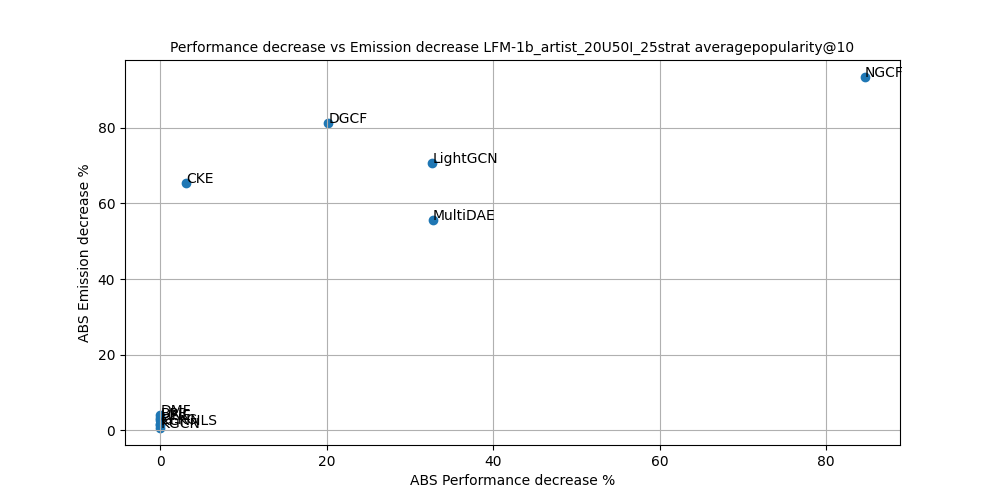
\includegraphics[scale=0.5]{images/decrement_averagepopularity@10_LFM-1b_artist_20U50I_25strat.png}
    \caption{Decremento di averagepopularity@10}
\end{figure}

\begin{figure}[H]
    \centering
    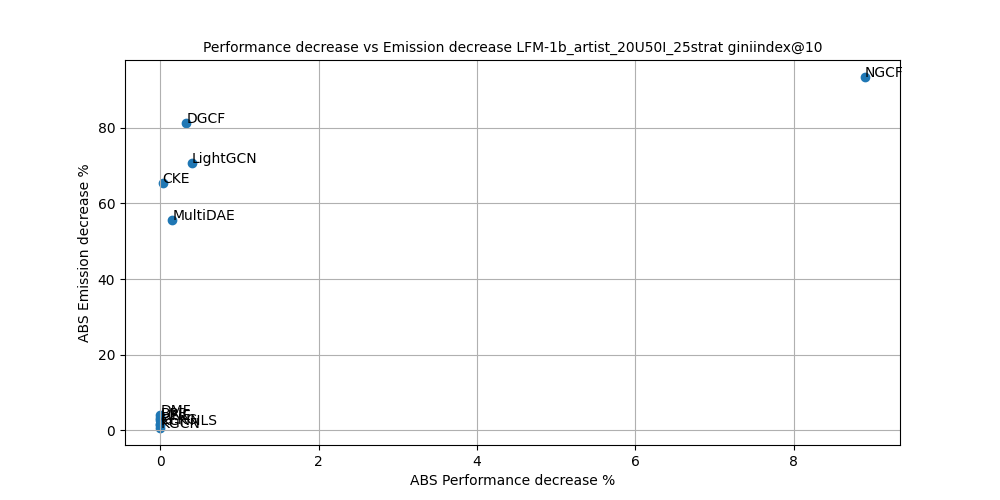
\includegraphics[scale=0.5]{images/decrement_giniindex@10_LFM-1b_artist_20U50I_25strat.png}
    \caption{Decremento di giniindex@10}
\end{figure}

\begin{figure}[H]
    \centering
    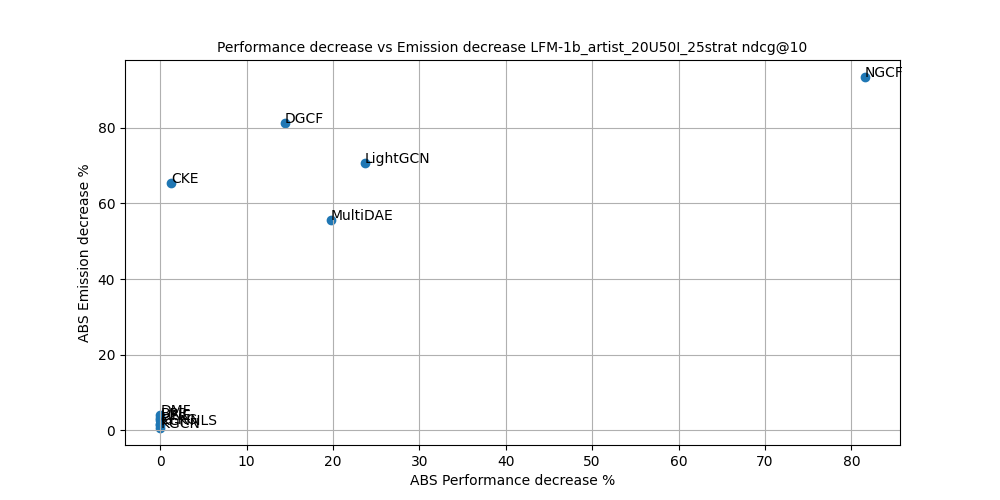
\includegraphics[scale=0.5]{images/decrement_ndcg@10_LFM-1b_artist_20U50I_25strat.png}
    \caption{Decremento di ndcg@10}
\end{figure}

\begin{figure}[H]
    \centering
    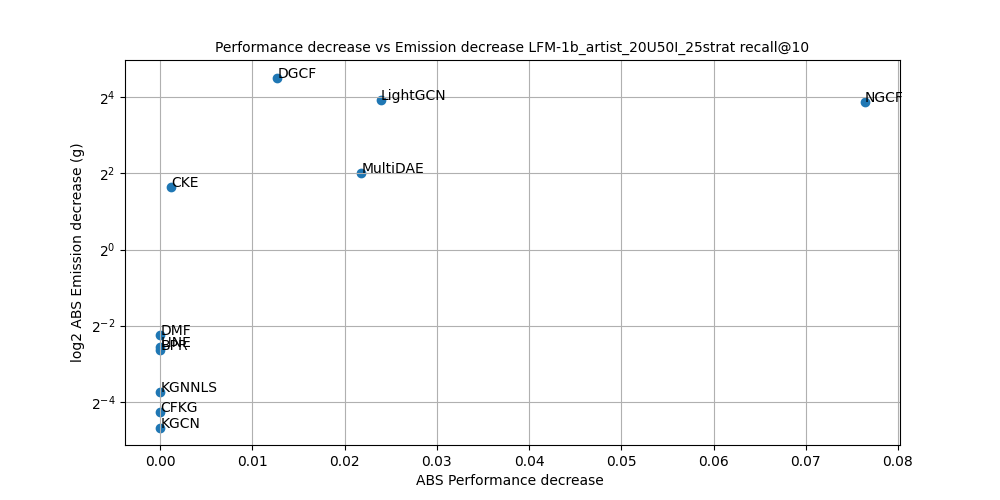
\includegraphics[scale=0.5]{images/decrement_recall@10_LFM-1b_artist_20U50I_25strat.png}
    \caption{Decremento di recall@10}
\end{figure}


\noindent Si può chiaramente notare come gli algoritmi che prima avevano registrato un aumento delle emissioni abbiano le stesse performance ad ogni metrica.
Questo è un chiaro segno che in questo caso gli algoritmi in entrambi i casi abbiano terminato l'esecuzione con il criterio di early stopping classico e che le emissioni abbiano subito un picco in un certo momento dovuto ad altri fattori.
Si può chiaramente notare come, rispetto al primo esperimento, tutti gli altri modelli, ad eccezione di NGCF, abbiano subito una riduzione delle performance molto più bassa rispetto al primo esperimento a fronte di riduzione di emissioni minori, a conferma che il criterio più stringente ha permesso a questi modelli di continuare l'addestramento e dunque essere allenati per più epoche.
Un anomalia si può notare per NGCF, che ha subito una riduzione delle performance molto alta rispetto al primo esperimento a fronte di una riduzione delle emissioni molto più alte. In entrambi i casi la differenza di errore è dell'ordine dei centesimi. Questo potrebbe essere dovuto al un dataset con diverse caratteristiche rispetto al precedente.

\subsubsection{Terzo esperimento}


Il terzo esperimento è stato eseguito sul dataset amazon\_books\_60core\_kg e i parametri utilizzati sono stati 40 come soglia e 6 come numero di epoche consecutive, dunque una via di mezzo tra i due esperimenti precedenti.

\begin{table}[H]
    \centering
    \footnotesize
    \setlength\tabcolsep{0pt}
    \begin{tabularx}{\textwidth}{|X|X|}
        \hline
        \textbf{Criterio classico} & \textbf{Criterio modificato} \\
        \hline
        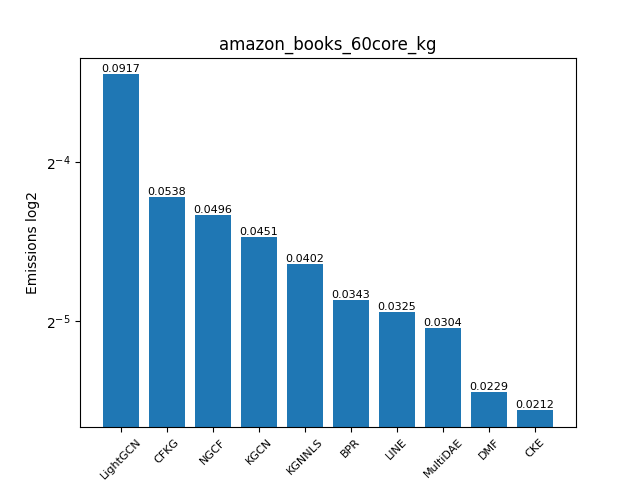
\includegraphics[width=\linewidth, trim=0 0 0 0]{images/emissions_amazon_books_60core_kg_earlyClassic.png} &
        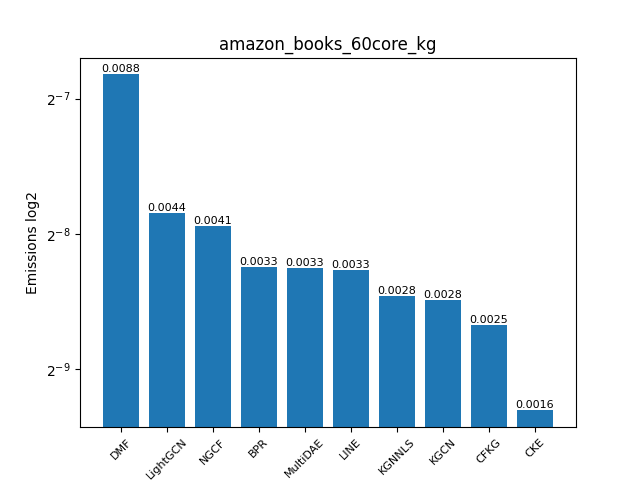
\includegraphics[width=\linewidth, trim=0 0 0 0]{images/emissions_amazon_books_60core_kg_earlyModified.png} \\
        \hline
    \end{tabularx}
    \caption{Emissioni con criterio classico e modificato}
    \label{tab:emissions_info}
\end{table}



\begin{table}[H]
    \centering
    \resizebox{\textwidth}{!}{
    \begin{tabular}{|c|c|c|c|}
        \hline
        \textbf{Modello} & \textbf{Emissioni criterio classico (g)} & \textbf{Emissioni criterio nuovo (g)} & \textbf{\% riduzione emissioni}\\
        \hline
        BPR & 34.3235 & 3.2958 & 90.398 \\
        \hline
        CKFG & 53.7798 & 2.4515 & 95.4416 \\
        \hline
        CKE & 21.1537 & 1.5824 & 92.5194 \\
        \hline
        DMF & 22.9403 & 8.8401 & 61.4649 \\
        \hline
        KGCN & 45.1294 & 2.7897 & 93.8185 \\
        \hline
        KGNNLS & 40.1533 & 2.8432 & 92.9192 \\
        \hline
        LINE & 32.5426 & 3.2539 & 90.0011 \\
        \hline
        MultiDAE & 30.3706 & 3.2749 & 89.2169 \\
        \hline
        LightGCN & 91.732 & 4.3526 & 95.2551 \\
        \hline
        NGCF & 49.55 & 4.0757 & 91.7745 \\
        \hline
    \end{tabular}
    }
    \caption{Confronto delle emissioni}
\end{table}

\noindent Come è possibile notare in questo caso la riduzione delle emissioni è molto alta per tutti i modelli, con valori che superano il 90\% per quasi tutti i modelli.


\begin{figure}[H]
    \centering
    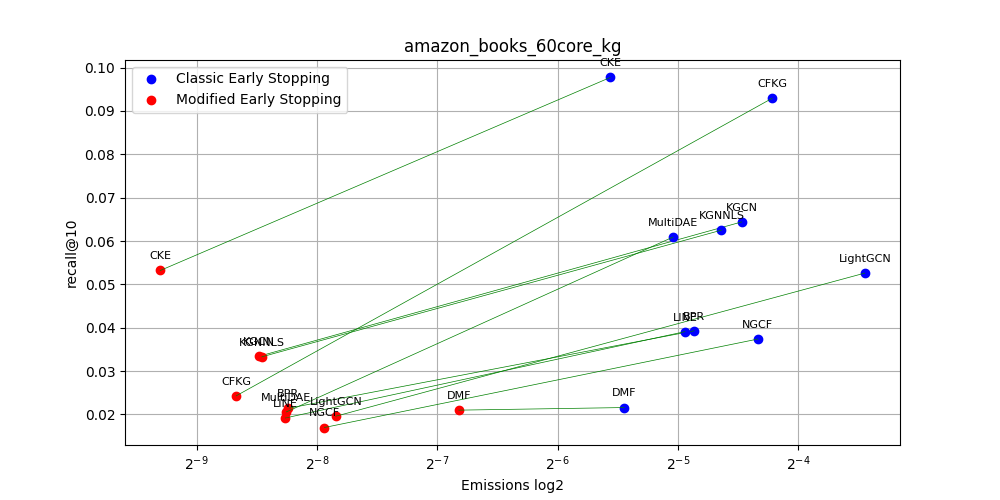
\includegraphics[width=\linewidth, trim=0 0 0 0]{images/recall@10_amazon_books_60core_kg_comparison.png}
    \caption{Confronto score recall@10 con dataset amazon\_books\_60core\_kg}
    
\end{figure}

\begin{figure}[H]
    \centering
    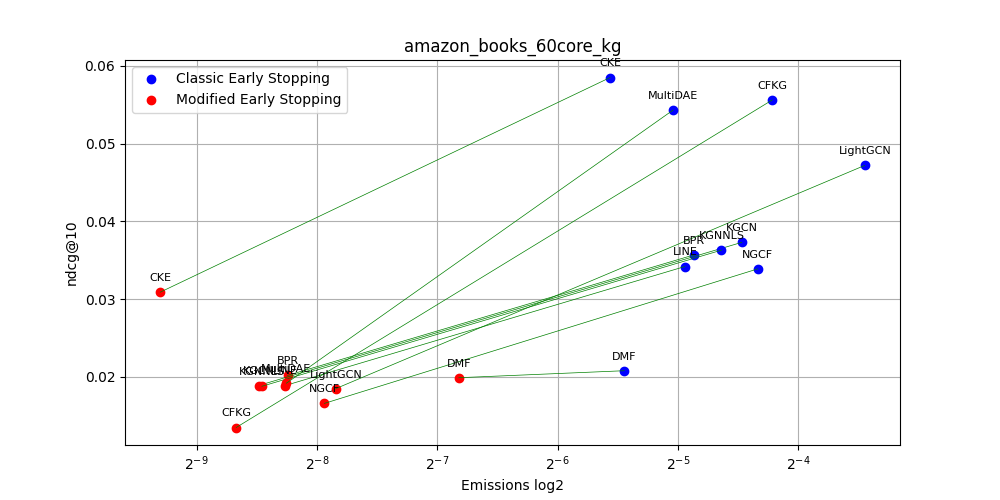
\includegraphics[width=\linewidth, trim=0 0 0 0]{images/ndcg@10_amazon_books_60core_kg_comparison.png}
    \caption{Confronto score ndcg@10 con dataset amazon\_books\_60core\_kg}
    
\end{figure}

\begin{figure}[H]
    \centering
    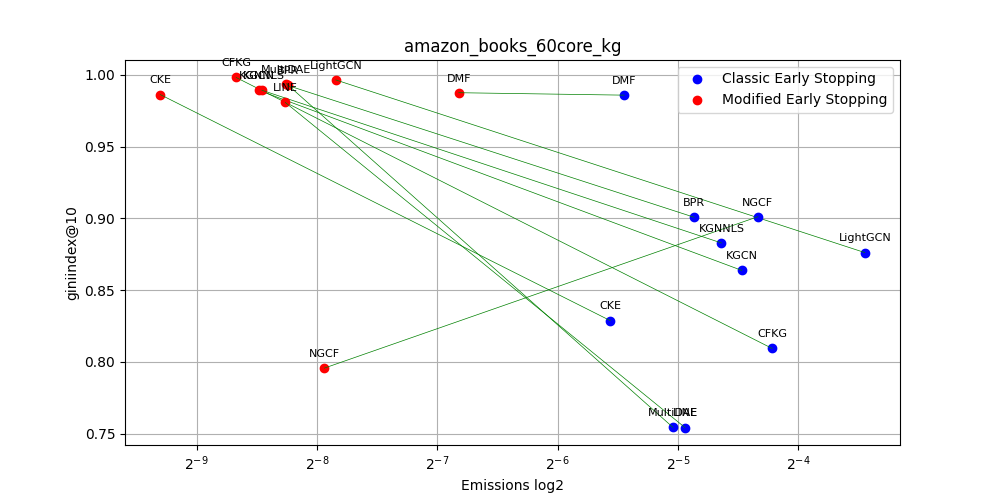
\includegraphics[width=\linewidth, trim=0 0 0 0]{images/giniindex@10_amazon_books_60core_kg_comparison.png}
    \caption{Confronto score giniindex@10 con dataset amazon\_books\_60core\_kg}
\end{figure}

\begin{figure}[H]
    \centering
    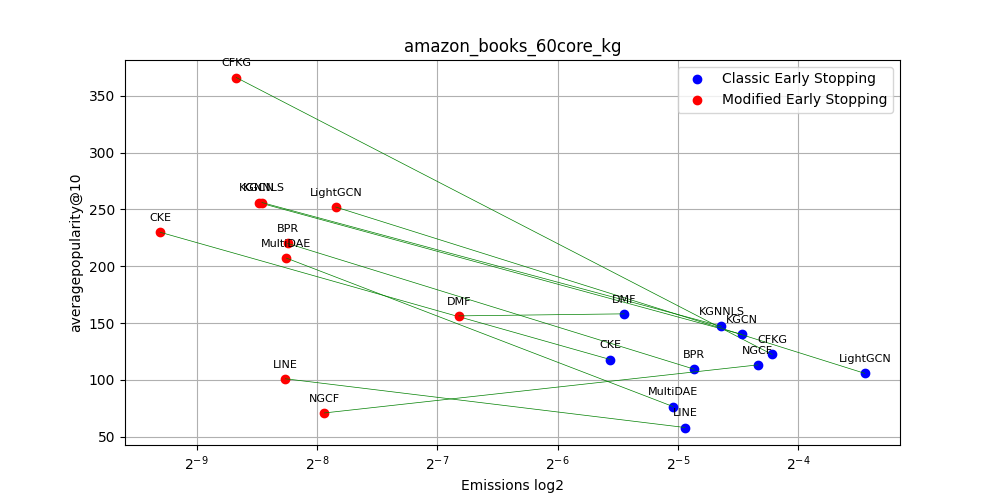
\includegraphics[width=\linewidth, trim=0 0 0 0]{images/averagepopularity@10_amazon_books_60core_kg_comparison.png}
    \caption{Confronto score averagepopularity@10 con dataset amazon\_books\_60core\_kg}
\end{figure}


\begin{table}[H]
    \centering
    \resizebox{\textwidth}{!}{
        \begin{tabular}{|c|c|c|c|c|}
    \hline
    \textbf{Modello} & \textbf{Metrica} & \textbf{Score criterio classico} & \textbf{Score criterio nuovo} & \textbf{\% riduzione score}\\
    \hline
    BPR              & recall@10         & 0.0393                        & 0.0214                          & 45.5471                               \\ \hline
    CFKG             & recall@10         & 0.0929                        & 0.0243                          & 73.8428                               \\ \hline
    CKE              & recall@10         & 0.0977                        & 0.0532                          & 45.5476                               \\ \hline
    DMF              & recall@10         & 0.0216                        & 0.021                           & 2.7778                                \\ \hline
    KGCN             & recall@10         & 0.0644                        & 0.0334                          & 48.1366                               \\ \hline
    KGNNLS           & recall@10         & 0.0625                        & 0.0333                          & 46.72                                 \\ \hline
    LINE             & recall@10         & 0.0391                        & 0.0192                          & 50.8951                               \\ \hline
    MultiDAE         & recall@10         & 0.0609                        & 0.0206                          & 66.1741                               \\ \hline
    LightGCN         & recall@10         & 0.0526                        & 0.0196                          & 62.7376                               \\ \hline
    NGCF             & recall@10         & 0.0374                        & 0.017                           & 54.5455                               \\ \hline
    BPR              & ndcg@10           & 0.0357                        & 0.0202                          & 43.4174                               \\ \hline
    CFKG             & ndcg@10           & 0.0556                        & 0.0135                          & 75.7194                               \\ \hline
    CKE              & ndcg@10           & 0.0585                        & 0.0309                          & 47.1795                               \\ \hline
    DMF              & ndcg@10           & 0.0208                        & 0.0199                          & 4.3269                                \\ \hline
    KGCN             & ndcg@10           & 0.0373                        & 0.0189                          & 49.3298                               \\ \hline
    KGNNLS           & ndcg@10           & 0.0363                        & 0.0188                          & 48.2094                               \\ \hline
    LINE             & ndcg@10           & 0.0342                        & 0.0189                          & 44.7368                               \\ \hline
    MultiDAE         & ndcg@10           & 0.0543                        & 0.0192                          & 64.6409                               \\ \hline
    LightGCN         & ndcg@10           & 0.0472                        & 0.0185                          & 60.8051                               \\ \hline
    NGCF             & ndcg@10           & 0.0339                        & 0.0166                          & 51.0324                               \\ \hline
    BPR              & avgpopularity@10 & 109.4148                      & 220.0387                        & -101.1051                             \\ \hline
    CFKG             & avgpopularity@10 & 122.3777                      & 366.0359                        & -199.1034                             \\ \hline
    CKE              & avgpopularity@10 & 117.927                       & 229.8594                        & -94.9167                              \\ \hline
    DMF              & avgpopularity@10 & 158.1008                      & 156.3042                        & 1.1364                                \\ \hline
    KGCN             & avgpopularity@10 & 140.0346                      & 256.0119                        & -82.8205                              \\ \hline
    KGNNLS           & avgpopularity@10 & 147.1768                      & 256.0278                        & -73.9593                              \\ \hline
    LINE             & avgpopularity@10 & 58.1057                       & 100.9865                        & -73.7979                              \\ \hline
    MultiDAE         & avgpopularity@10 & 76.5618                       & 207.1265                        & -170.535                              \\ \hline
    LightGCN         & avgpopularity@10 & 105.7397                      & 252.0464                        & -138.365                              \\ \hline
    NGCF             & avgpopularity@10 & 113.2036                      & 70.9028                         & 37.367                                \\ \hline
    BPR              & giniindex@10     & 0.9007                        & 0.9926                          & -10.2032                              \\ \hline
    CFKG             & giniindex@10     & 0.8093                        & 0.9981                          & -23.3288                              \\ \hline
    CKE              & giniindex@10     & 0.8287                        & 0.9862                          & -19.0057                              \\ \hline
    DMF              & giniindex@10     & 0.9858                        & 0.9875                          & -0.1724                               \\ \hline
    KGCN             & giniindex@10     & 0.8637                        & 0.9892                          & -14.5305                              \\ \hline
    KGNNLS           & giniindex@10     & 0.8828                        & 0.9892                          & -12.0526                              \\ \hline
    LINE             & giniindex@10     & 0.7542                        & 0.9807                          & -30.0318                              \\ \hline
    MultiDAE         & giniindex@10     & 0.7543                        & 0.9938                          & -31.7513                              \\ \hline
    LightGCN         & giniindex@10     & 0.8761                        & 0.9964                          & -13.7313                              \\ \hline
    NGCF             & giniindex@10     & 0.9011                        & 0.7956                          & 11.7079                               \\ \hline
    \end{tabular}
    }
    \caption{Performance dei modelli su diverse metriche e dataset}
    \end{table}


\begin{figure}[H]
    \centering
    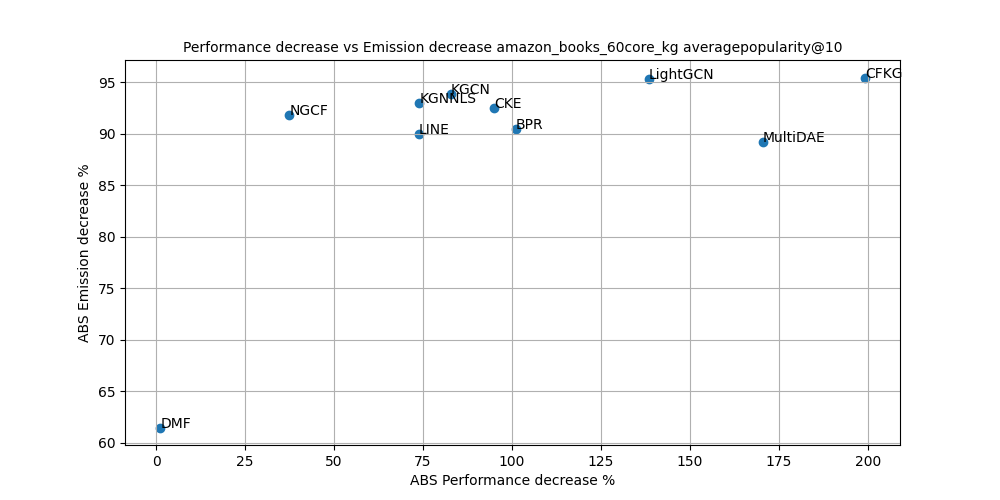
\includegraphics[scale=0.5]{images/decrement_averagepopularity@10_amazon_books_60core_kg.png}
    \caption{Decremento di averagepopularity@10}
\end{figure}

\begin{figure}[H]
    \centering
    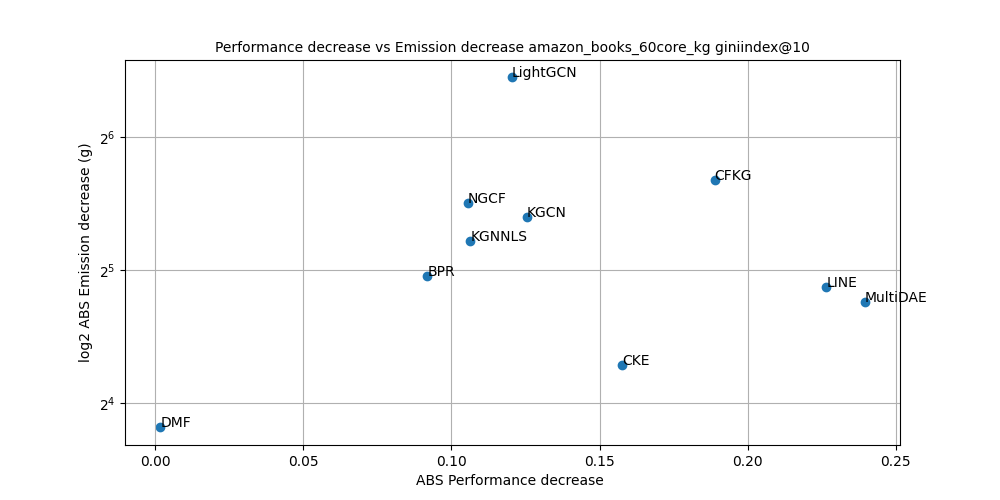
\includegraphics[scale=0.5]{images/decrement_giniindex@10_amazon_books_60core_kg.png}
    \caption{Decremento di giniindex@10}
\end{figure}

\begin{figure}[H]
    \centering
    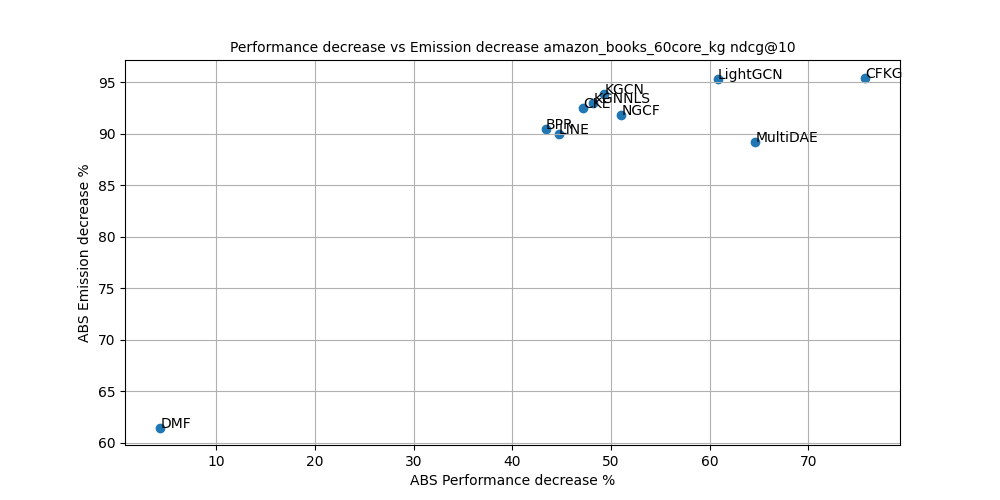
\includegraphics[scale=0.5]{images/decrement_ndcg@10_amazon_books_60core_kg.png}
    \caption{Decremento di ndcg@10}
\end{figure}

\begin{figure}[H]
    \centering
    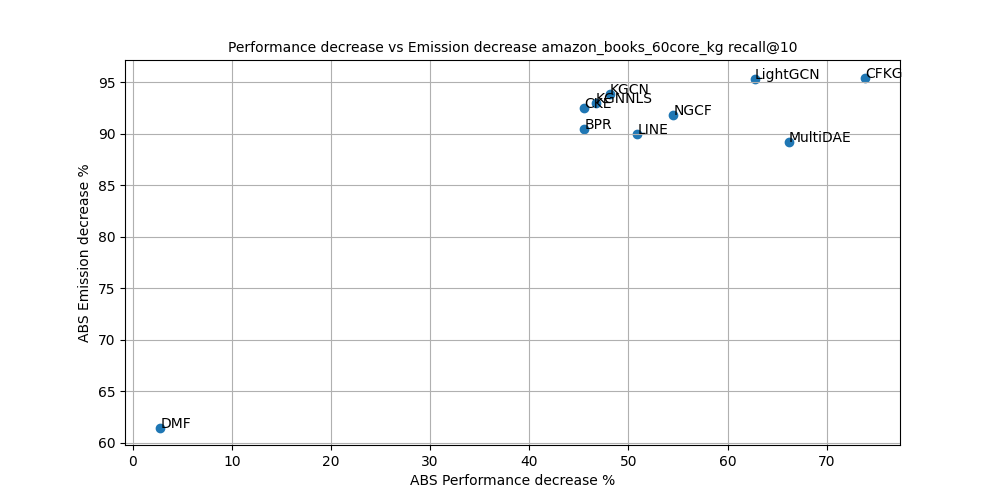
\includegraphics[scale=0.5]{images/decrement_recall@10_amazon_books_60core_kg.png}
    \caption{Decremento di recall@10}
\end{figure}
\noindent Si può notare come le forti riduzioni di emissioni abbiano portato a una riduzione delle performance molto più alta rispetto ai due esperimenti precedenti.
DMF è l'unico modello che ha mantenuto performance quasi invarianti a fronte di una riduzione delle emissioni del 61\%. (la più bassa ma comunque molto alta).
    

\subsection{Confronto tra criteri}
La parte esplorativa ha mostrato come alcuni algoritmi (DGCF per esempio) mostrino un'elevata riduzione delle performance in ogni contesto, mentre alti come DFM rimangono stabili.
Tenendo conto dei parametri utilizzati e delle dimensioni dei dataset è evidente come all'aumentare della dimensione del dataset bisogna diminuire la soglia di tollereanza e aumentare il numero di epoche consecutive per ottenere emissioni ridotte senza perdere troppo in performance.
Seguiranno dunque diversi risultati eseguiti con il dataset MovieLens-1m

\subsubsection{Primo esperimento}
Il primo esperimento è stato effettuato con una soglia di tolleranza pari a 40 e un numero di epoche consecutive pari a 5

\begin{table}[H]
    \centering
    \footnotesize
    \setlength\tabcolsep{0pt}
    \begin{tabularx}{\textwidth}{|X|X|}
        \hline
        \textbf{Criterio classico} & \textbf{Criterio modificato} \\
        \hline
        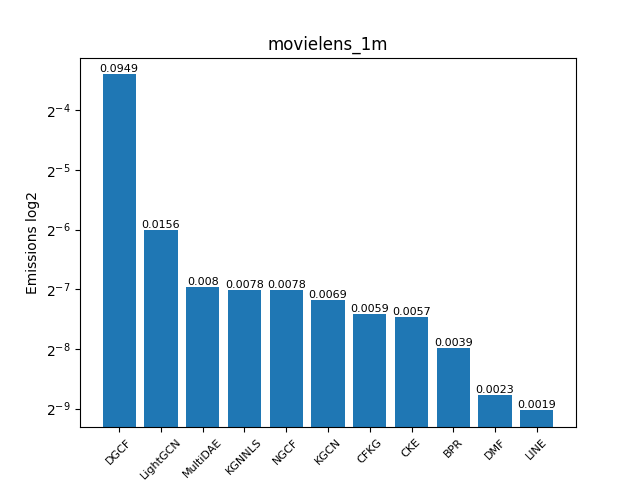
\includegraphics[width=\linewidth, trim=0 0 0 0]{images/emissions_movielens_1m_40_5_earlyClassic.png} &
        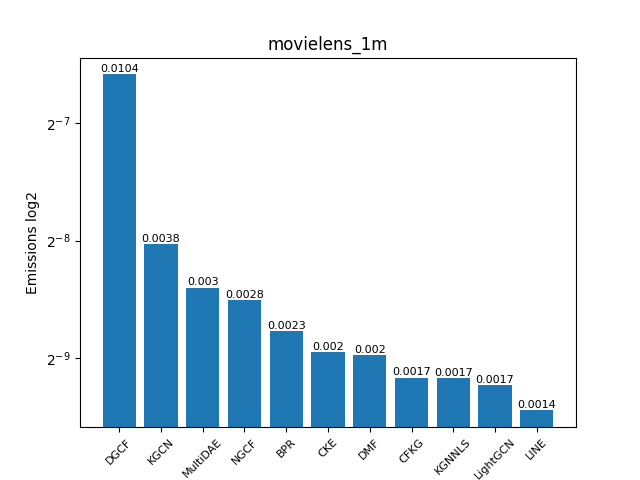
\includegraphics[width=\linewidth, trim=0 0 0 0]{images/emissions_movielens_1m_40_5_earlyModified.png} \\
        \hline
    \end{tabularx}
    \caption{Emissioni con criterio classico e modificato}
    \label{tab:emissions_info}
\end{table}



\begin{table}[H]
    \centering
    \resizebox{\textwidth}{!}{
    \begin{tabular}{|c|c|c|c|}
        \hline
        \textbf{Modello} & \textbf{Emissioni criterio classico (g)} & \textbf{Emissioni criterio nuovo (g)} & \textbf{\% riduzione emissioni}\\
        \hline
        BPR & 3.9484 & 2.2898 & 42.0068 \\ \hline
        CKFG & 5.881 & 1.7411 & 70.3944 \\ \hline
        CKE & 5.6839 & 2.0271 & 64.3357 \\ \hline
        DMF & 2.2927 & 1.9885 & 13.2688 \\ \hline
        KGCN & 6.8754 & 3.8305 & 44.2875 \\ \hline
        KGNNLS & 7.763 & 1.7384 & 77.607 \\ \hline
        LINE & 1.9129 & 1.4341 & 25.0296 \\ \hline
        MultiDAE & 8.0303 & 2.9614 & 63.68 \\ \hline
        LightGCN & 15.626 & 1.6634 & 89.3547 \\ \hline
        NGCF & 7.7582 & 2.7574 & 64.4576 \\ \hline
        DGCF & 94.903 & 10.4183 & 89.0222 \\ \hline

    \end{tabular}
    }
    \caption{Confronto delle emissioni}
\end{table}

\noindent Rispetto all'ultimo esperimento con lo stesso dataset, possiamo notare come la sola riduzione della soglia da 50 a 40 abbia portato molti algoritmi e diminuire la percentuale di riduzione delle emissioni, mentre per tanti altri la percentuale è pressocchè invariata

\begin{figure}[H]
    \centering
    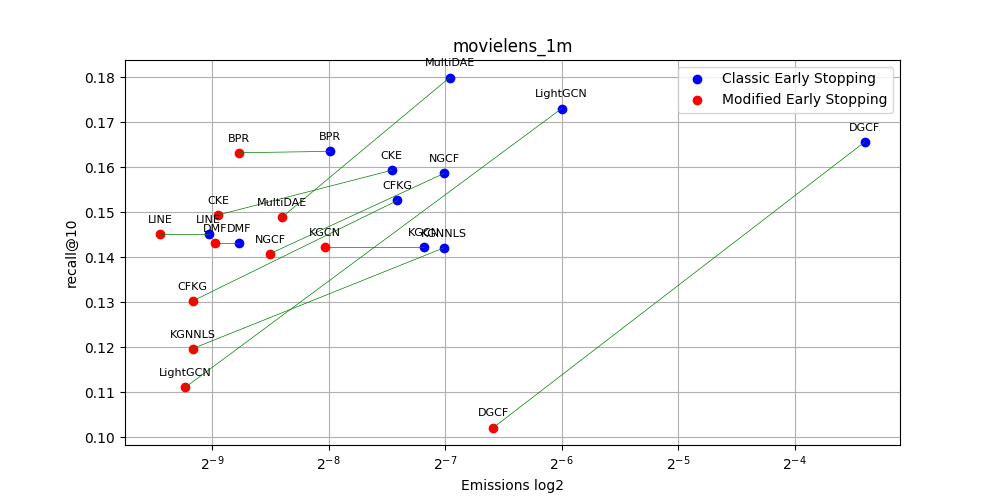
\includegraphics[width=\linewidth, trim=0 0 0 0]{images/recall@10_movielens_1m_40_5_comparison.png}
    \caption{Confronto score recall@10}
    
\end{figure}

\begin{figure}[H]
    \centering
    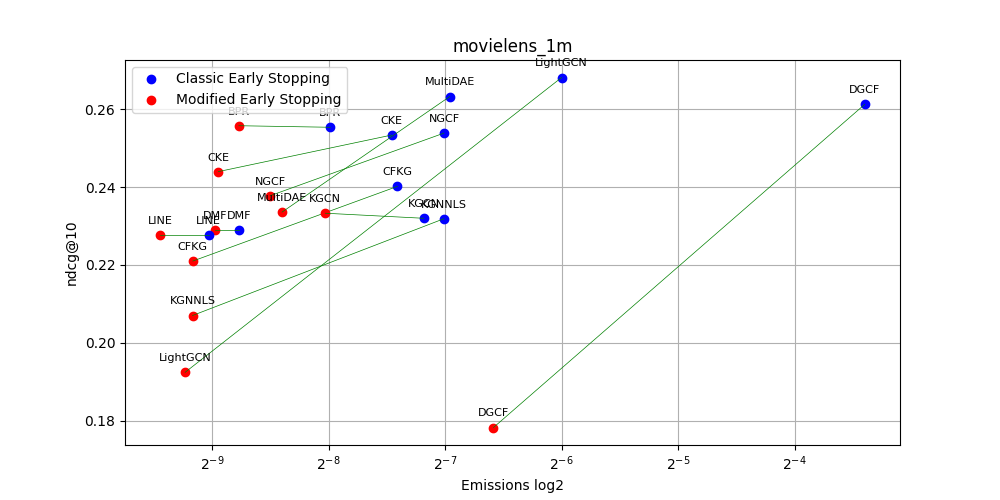
\includegraphics[width=\linewidth, trim=0 0 0 0]{images/ndcg@10_movielens_1m_40_5_comparison.png}
    \caption{Confronto score ndcg@10}
    
\end{figure}

\begin{figure}[H]
    \centering
    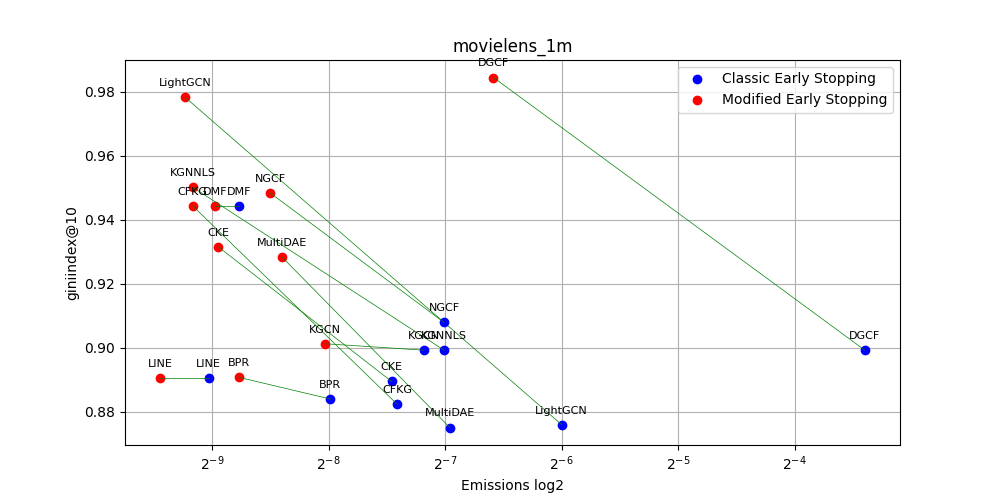
\includegraphics[width=\linewidth, trim=0 0 0 0]{images/giniindex@10_movielens_1m_40_5_comparison.png}
    \caption{Confronto score giniindex@10}
\end{figure}

\begin{figure}[H]
    \centering
    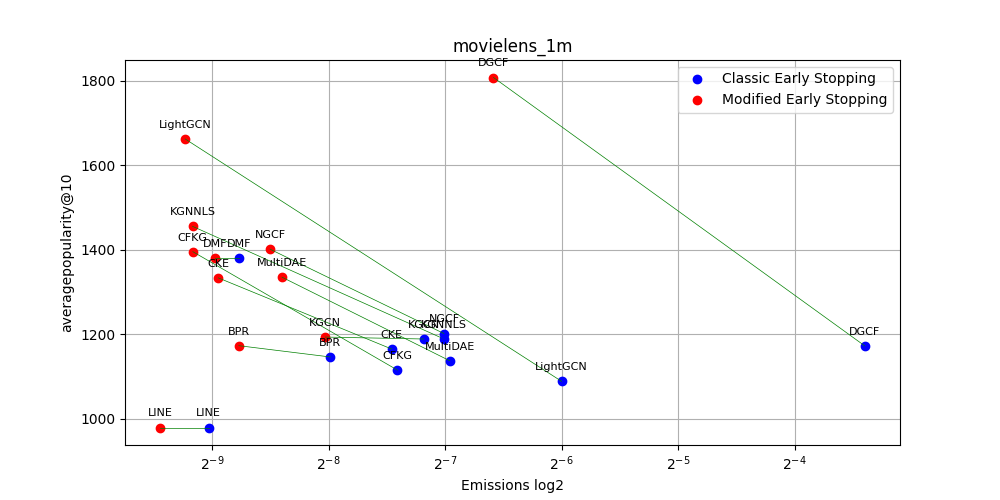
\includegraphics[width=\linewidth, trim=0 0 0 0]{images/averagepopularity@10_movielens_1m_40_5_comparison.png}
    \caption{Confronto score averagepopularity@10}
\end{figure}


\begin{table}[H]
    \centering
    \resizebox{\textwidth}{!}{
        \begin{tabular}{|c|c|c|c|c|}
    \hline
    \textbf{Modello} & \textbf{Metrica} & \textbf{Score criterio classico} & \textbf{Score criterio nuovo} & \textbf{\% riduzione score}\\
    \hline
BPR              & recall@10         & 0.1635                        & 0.1632                           & 0.1835                               \\ \hline
CFKG             & recall@10         & 0.1526                        & 0.1303                           & 14.6134                              \\ \hline
CKE              & recall@10         & 0.1593                        & 0.1494                           & 6.2147                               \\ \hline
DMF              & recall@10         & 0.1432                        & 0.1432                           & 0.0                                  \\ \hline
KGCN             & recall@10         & 0.1422                        & 0.1422                           & 0.0                                  \\ \hline
KGNNLS           & recall@10         & 0.1421                        & 0.1197                           & 15.7635                              \\ \hline
LINE             & recall@10         & 0.1451                        & 0.1451                           & 0.0                                  \\ \hline
MultiDAE         & recall@10         & 0.1799                        & 0.1489                           & 17.2318                              \\ \hline
LightGCN         & recall@10         & 0.173                         & 0.1111                           & 35.7803                              \\ \hline
NGCF             & recall@10         & 0.1586                        & 0.1408                           & 11.2232                              \\ \hline
DGCF             & recall@10         & 0.1656                        & 0.1022                           & 38.285                               \\ \hline
BPR              & ndcg@10           & 0.2554                        & 0.2558                           & -0.1566                              \\ \hline
CFKG             & ndcg@10           & 0.2402                        & 0.221                            & 7.9933                               \\ \hline
CKE              & ndcg@10           & 0.2534                        & 0.244                            & 3.7096                               \\ \hline
DMF              & ndcg@10           & 0.2289                        & 0.2289                           & 0.0                                  \\ \hline
KGCN             & ndcg@10           & 0.232                         & 0.2333                           & -0.5603                              \\ \hline
KGNNLS           & ndcg@10           & 0.2319                        & 0.207                            & 10.7374                              \\ \hline
LINE             & ndcg@10           & 0.2277                        & 0.2277                           & 0.0                                  \\ \hline
MultiDAE         & ndcg@10           & 0.2633                        & 0.2336                           & 11.2799                              \\ \hline
LightGCN         & ndcg@10           & 0.2682                        & 0.1924                           & 28.2625                              \\ \hline
NGCF             & ndcg@10           & 0.2539                        & 0.2378                           & 6.3411                               \\ \hline
DGCF             & ndcg@10           & 0.2613                        & 0.1782                           & 31.8025                              \\ \hline
BPR              & avgpopularity@10 & 1146.3572                     & 1173.1199                        & -2.3346                              \\ \hline
CFKG             & avgpopularity@10 & 1115.4498                     & 1395.6098                        & -25.1163                             \\ \hline
CKE              & avgpopularity@10 & 1165.2413                     & 1333.5153                        & -14.4411                             \\ \hline
DMF              & avgpopularity@10 & 1379.7292                     & 1379.7292                        & 0.0                                  \\ \hline
KGCN             & avgpopularity@10 & 1188.9582                     & 1193.5298                        & -0.3845                              \\ \hline
KGNNLS           & avgpopularity@10 & 1188.8981                     & 1455.58                          & -22.431                              \\ \hline
LINE             & avgpopularity@10 & 979.498                       & 979.498                          & 0.0                                  \\ \hline
MultiDAE         & avgpopularity@10 & 1137.4597                     & 1335.1498                        & -17.38                               \\ \hline
LightGCN         & avgpopularity@10 & 1088.741                      & 1662.4263                        & -52.6925                             \\ \hline
NGCF             & avgpopularity@10 & 1201.8831                     & 1401.4325                        & -16.6031                             \\ \hline
DGCF             & avgpopularity@10 & 1172.6874                     & 1807.8717                        & -54.1648                             \\ \hline
BPR              & giniindex@10     & 0.8839                        & 0.8907                           & -0.7693                              \\ \hline
CFKG             & giniindex@10     & 0.8822                        & 0.9443                           & -7.0392                              \\ \hline
CKE              & giniindex@10     & 0.8894                        & 0.9315                           & -4.7335                              \\ \hline
DMF              & giniindex@10     & 0.9443                        & 0.9443                           & 0.0                                  \\ \hline
KGCN             & giniindex@10     & 0.8992                        & 0.9012                           & -0.2224                              \\ \hline
KGNNLS           & giniindex@10     & 0.8992                        & 0.9502                           & -5.6717                              \\ \hline
LINE             & giniindex@10     & 0.8904                        & 0.8904                           & 0.0                                  \\ \hline
MultiDAE         & giniindex@10     & 0.875                         & 0.9283                           & -6.0914                              \\ \hline
LightGCN         & giniindex@10     & 0.8759                        & 0.9783                           & -11.6908                             \\ \hline
NGCF             & giniindex@10     & 0.9079                        & 0.9484                           & -4.4608                              \\ \hline
DGCF             & giniindex@10     & 0.8992                        & 0.9845                           & -9.4862                              \\ \hline
\end{tabular}
    }
    \caption{Performance dei modelli su diverse metriche e dataset}
    \end{table}


\begin{figure}[H]
    \centering
    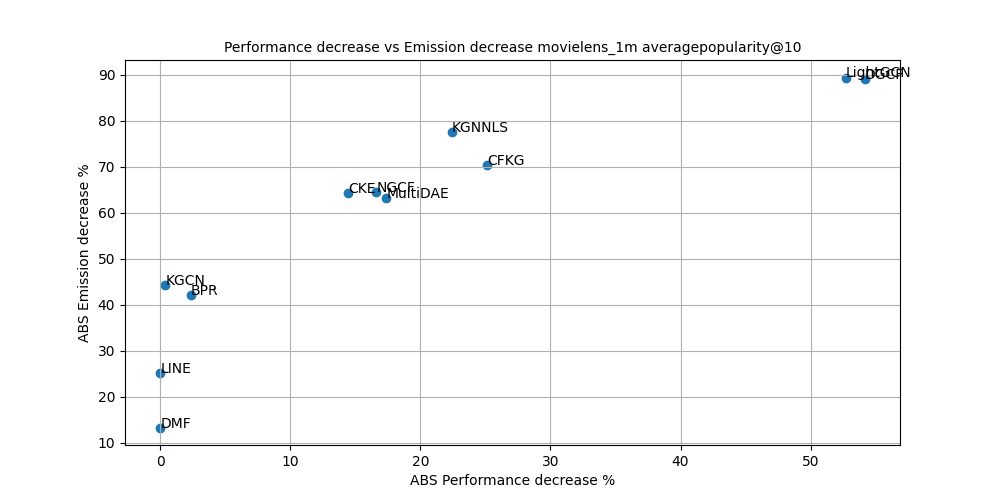
\includegraphics[scale=0.5]{images/decrement_averagepopularity@10_movielens_1m_40_5.png}
    \caption{Decremento di averagepopularity@10}
\end{figure}

\begin{figure}[H]
    \centering
    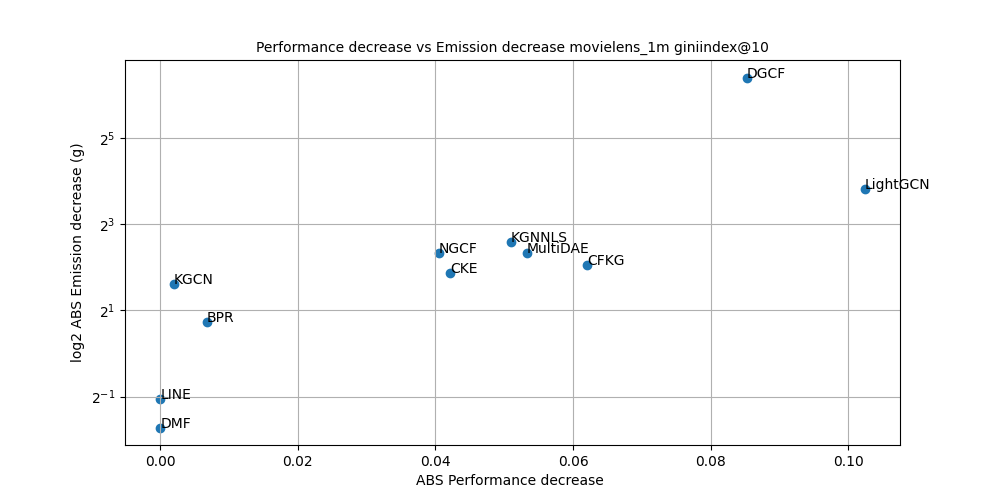
\includegraphics[scale=0.5]{images/decrement_giniindex@10_movielens_1m_40_5.png}
    \caption{Decremento di giniindex@10}
\end{figure}

\begin{figure}[H]
    \centering
    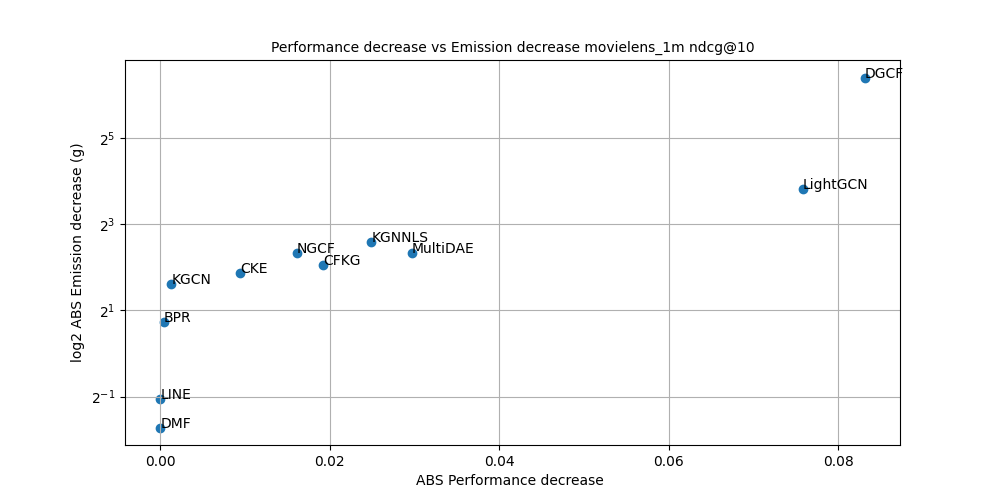
\includegraphics[scale=0.5]{images/decrement_ndcg@10_movielens_1m_40_5.png}
    \caption{Decremento di ndcg@10}
\end{figure}

\begin{figure}[H]
    \centering
    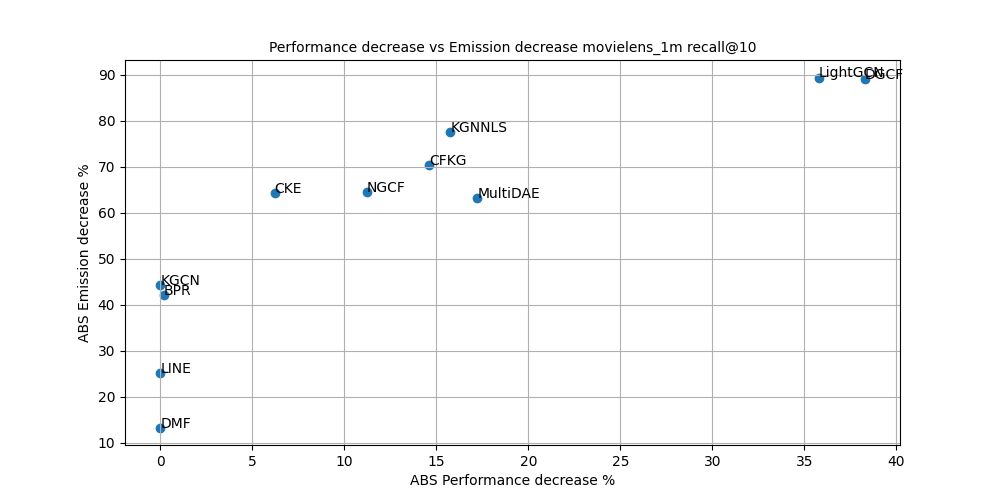
\includegraphics[scale=0.5]{images/decrement_recall@10_movielens_1m_40_5.png}
    \caption{Decremento di recall@10}
\end{figure}
\noindent Il calo delle performance è più contenuto rispetto all'esperimento precedente. Anche in questo caso per molti modelli la riduzione delle performance è pressocchè identica rispetto all'esperimento precedente, per pochi modelli invece la riduzione delle performance è inferiore


\subsubsection{Secondo esperimento}
Il secondo esperimento è stato effettuato con una soglia di tolleranza pari a 30 e un numero di epoche consecutive pari a 5 (dunque criterio più stringente rispetto al primo esperimento)

\begin{table}[H]
    \centering
    \footnotesize
    \setlength\tabcolsep{0pt}
    \begin{tabularx}{\textwidth}{|X|X|}
        \hline
        \textbf{Criterio classico} & \textbf{Criterio modificato} \\
        \hline
        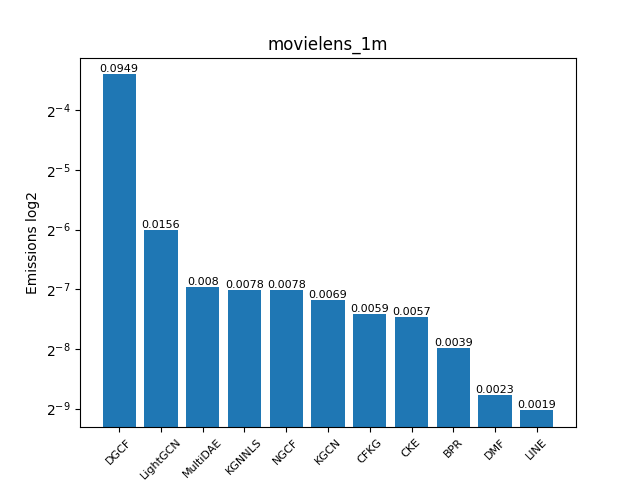
\includegraphics[width=\linewidth, trim=0 0 0 0]{images/emissions_movielens_1m_30_5_earlyClassic.png} &
        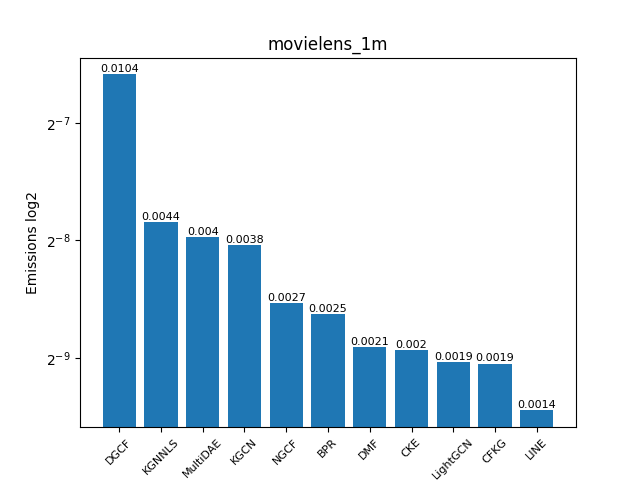
\includegraphics[width=\linewidth, trim=0 0 0 0]{images/emissions_movielens_1m_30_5_earlyModified.png} \\
        \hline
    \end{tabularx}
    \caption{Emissioni con criterio classico e modificato}
    \label{tab:emissions_info}
\end{table}



\begin{table}[H]
    \centering
    \resizebox{\textwidth}{!}{
    \begin{tabular}{|c|c|c|c|}
        \hline
        \textbf{Modello} & \textbf{Emissioni criterio classico (g)} & \textbf{Emissioni criterio nuovo (g)} & \textbf{\% riduzione emissioni}\\
        \hline
        BPR & 3.9484 & 2.5219 & 36.1284 \\ \hline
        CKFG & 5.881 & 1.8872 & 67.9104 \\ \hline
        CKE & 5.6839 & 2.0466 & 63.9932 \\ \hline
        DMF & 2.2927 & 2.0856 & 9.0319 \\ \hline
        KGCN & 6.8754 & 3.796 & 44.7884 \\ \hline
        KGNNLS & 7.763 & 4.3657 & 43.7626 \\ \hline
        LINE & 1.9129 & 1.4314 & 25.1721 \\ \hline
        MultiDAE & 8.0303 & 3.9614 & 50.4865 \\ \hline
        LightGCN & 15.626 & 1.9001 & 87.8402 \\ \hline
        NGCF & 7.7582 & 2.6923 & 65.2979 \\ \hline
        DGCF & 94.903 & 10.4109 & 89.03 \\ \hline

    \end{tabular}
    }
    \caption{Confronto delle emissioni}
\end{table}

\noindent Rispetto al primo esperimento si può facilemnte notare come una soglia più bassa abbia portato a un generale diminuzione della percentuale di riduzione delle emissioni (cioè gli algoritmi hanno eseguito un training più lungo).


\begin{figure}[H]
    \centering
    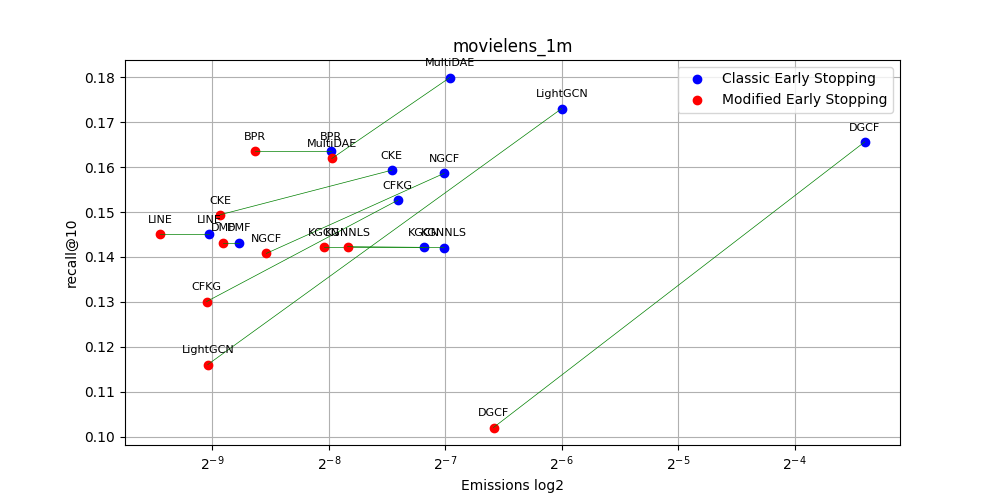
\includegraphics[width=\linewidth, trim=0 0 0 0]{images/recall@10_movielens_1m_30_5_comparison.png}
    \caption{Confronto score recall@10}
    
\end{figure}

\begin{figure}[H]
    \centering
    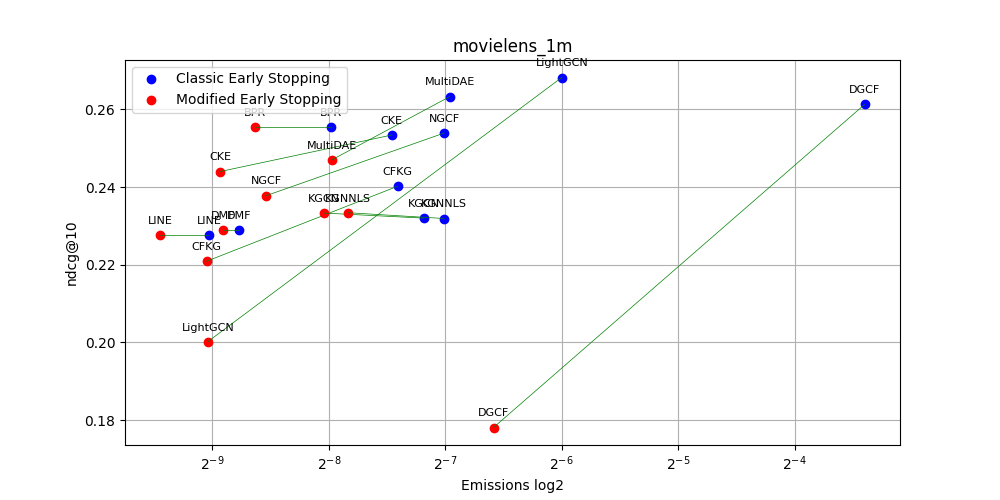
\includegraphics[width=\linewidth, trim=0 0 0 0]{images/ndcg@10_movielens_1m_30_5_comparison.png}
    \caption{Confronto score ndcg@10}
    
\end{figure}

\begin{figure}[H]
    \centering
    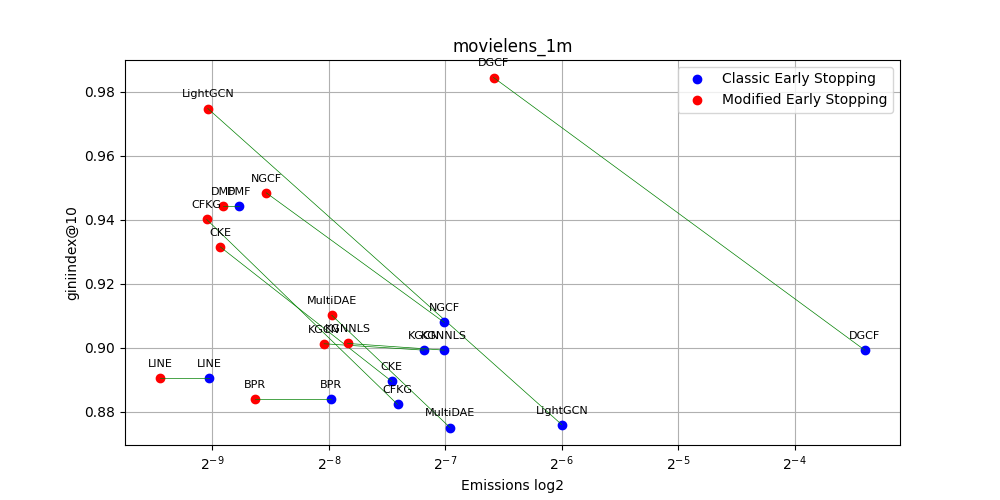
\includegraphics[width=\linewidth, trim=0 0 0 0]{images/giniindex@10_movielens_1m_30_5_comparison.png}
    \caption{Confronto score giniindex@10}
\end{figure}

\begin{figure}[H]
    \centering
    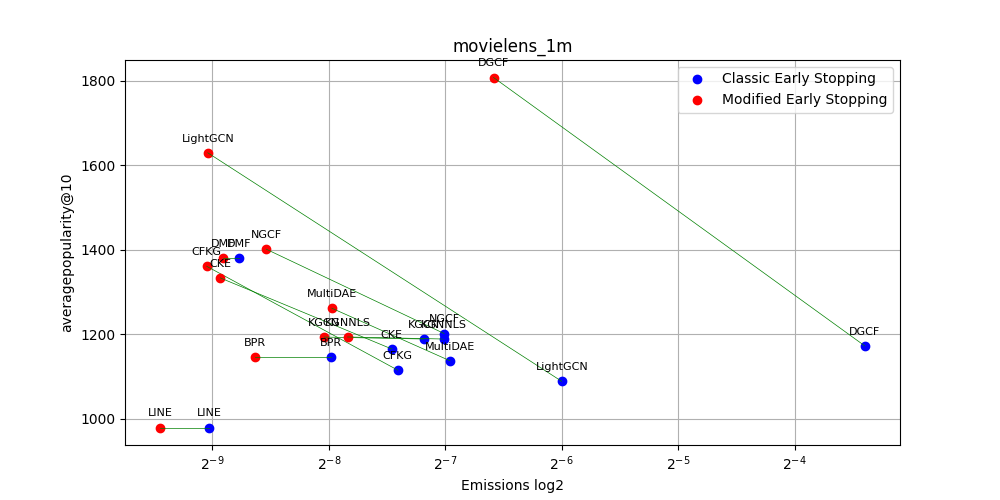
\includegraphics[width=\linewidth, trim=0 0 0 0]{images/averagepopularity@10_movielens_1m_30_5_comparison.png}
    \caption{Confronto score averagepopularity@10}
\end{figure}


\begin{table}[H]
    \centering
    \resizebox{\textwidth}{!}{
        \begin{tabular}{|c|c|c|c|c|}
    \hline
    \textbf{Modello} & \textbf{Metrica} & \textbf{Score criterio classico} & \textbf{Score criterio nuovo} & \textbf{\% riduzione score}\\
    \hline
    BPR & recall@10 & 0.1635 & 0.1635 & 0.0 \\ \hline
    CFKG & recall@10 & 0.1526 & 0.1301 & 14.7444 \\ \hline
    CKE & recall@10 & 0.1593 & 0.1494 & 6.2147 \\ \hline
    DMF & recall@10 & 0.1432 & 0.1432 & 0.0 \\ \hline 
    KGCN & recall@10 & 0.1422 & 0.1422 & 0.0 \\ \hline
    KGNNLS & recall@10 & 0.1421 & 0.1423 & -0.1407 \\ \hline
    LINE & recall@10 & 0.1451 & 0.1451 & 0.0 \\ \hline
    MultiDAE & recall@10 & 0.1799 & 0.1619 & 10.0056 \\ \hline
    LightGCN & recall@10 & 0.173 & 0.1161 & 32.8902 \\ \hline
    NGCF & recall@10 & 0.1586 & 0.1408 & 11.2232 \\ \hline
    DGCF & recall@10 & 0.1656 & 0.1021 & 38.3454 \\ \hline
    BPR & ndcg@10 & 0.2554 & 0.2554 & 0.0 \\ \hline
    CFKG & ndcg@10 & 0.2402 & 0.2209 & 8.035 \\ \hline
    CKE & ndcg@10 & 0.2534 & 0.244 & 3.7096 \\      \hline
    DMF & ndcg@10 & 0.2289 & 0.2289 & 0.0 \\\hline
    KGCN & ndcg@10 & 0.232 & 0.2333 & -0.5603 \\\hline
    KGNNLS & ndcg@10 & 0.2319 & 0.2334 & -0.6468 \\\hline
    LINE & ndcg@10 & 0.2277 & 0.2277 & 0.0 \\\hline
    MultiDAE & ndcg@10 & 0.2633 & 0.247 & 6.1907 \\\hline
    LightGCN & ndcg@10 & 0.2682 & 0.2002 & 25.3542 \\\hline
    NGCF & ndcg@10 & 0.2539 & 0.2378 & 6.3411 \\\hline
    DGCF & ndcg@10 & 0.2613 & 0.1781 & 31.8408 \\ \hline
    BPR & averagepopularity@10 & 1146.3572 & 1146.3572 & 0.0 \\\hline
    CFKG & averagepopularity@10 & 1115.4498 & 1361.1447 & -22.0265 \\\hline
    CKE & averagepopularity@10 & 1165.2413 & 1333.5153 & -14.4411 \\\hline
    DMF & averagepopularity@10 & 1379.7292 & 1379.7292 & 0.0 \\\hline
    KGCN & averagepopularity@10 & 1188.9582 & 1193.5298 & -0.3845 \\\hline
    KGNNLS & averagepopularity@10 & 1188.8981 & 1193.7263 & -0.4061 \\\hline
    LINE & averagepopularity@10 & 979.498 & 979.498 & 0.0 \\\hline
    MultiDAE & averagepopularity@10 & 1137.4597 & 1261.7868 & -10.9302 \\\hline
    LightGCN & averagepopularity@10 & 1088.741 & 1629.6349 & -49.6807 \\\hline
    NGCF & averagepopularity@10 & 1201.8831 & 1401.4325 & -16.6031 \\\hline
    DGCF & averagepopularity@10 & 1172.6874 & 1807.9008 & -54.1673 \\ \hline
    BPR & giniindex@10 & 0.8839 & 0.8839 & 0.0 \\\hline
    CFKG & giniindex@10 & 0.8822 & 0.9401 & -6.5631 \\\hline
    CKE & giniindex@10 & 0.8894 & 0.9315 & -4.7335 \\\hline
    DMF & giniindex@10 & 0.9443 & 0.9443 & 0.0 \\\hline
    KGCN & giniindex@10 & 0.8992 & 0.9012 & -0.2224 \\\hline
    KGNNLS & giniindex@10 & 0.8992 & 0.9013 & -0.2335 \\\hline
    LINE & giniindex@10 & 0.8904 & 0.8904 & 0.0 \\\hline
    MultiDAE & giniindex@10 & 0.875 & 0.9101 & -4.0114 \\\hline
    LightGCN & giniindex@10 & 0.8759 & 0.9748 & -11.2912 \\\hline
    NGCF & giniindex@10 & 0.9079 & 0.9484 & -4.4608 \\\hline
    DGCF & giniindex@10 & 0.8992 & 0.9845 & -9.4862 \\ \hline
\end{tabular}
    }
    \caption{Performance dei modelli su diverse metriche e dataset}
    \end{table}


\begin{figure}[H]
    \centering
    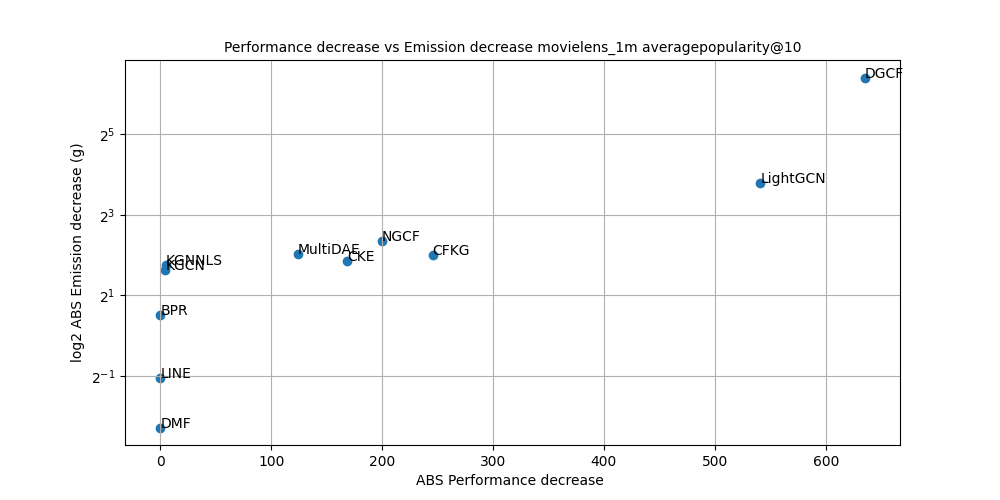
\includegraphics[scale=0.5]{images/decrement_averagepopularity@10_movielens_1m_30_5.png}
    \caption{Decremento di averagepopularity@10}
\end{figure}

\begin{figure}[H]
    \centering
    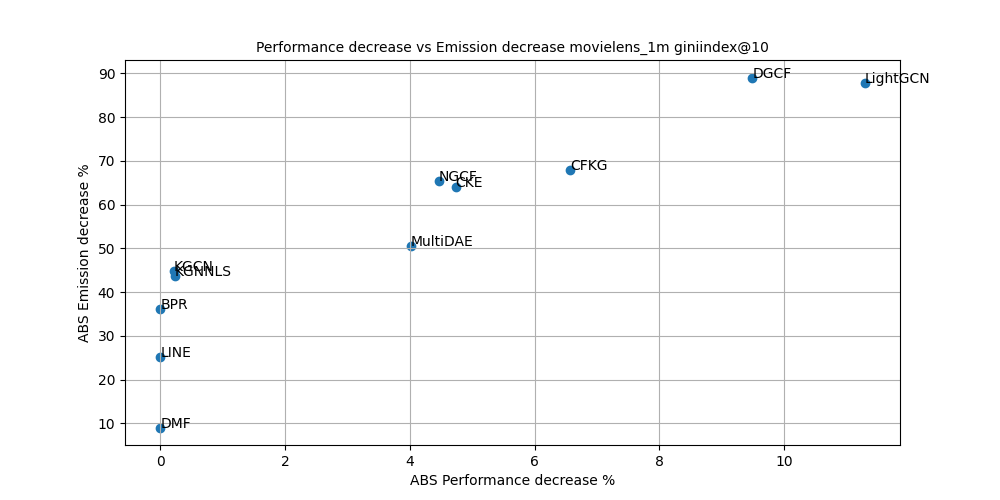
\includegraphics[scale=0.5]{images/decrement_giniindex@10_movielens_1m_30_5.png}
    \caption{Decremento di giniindex@10}
\end{figure}

\begin{figure}[H]
    \centering
    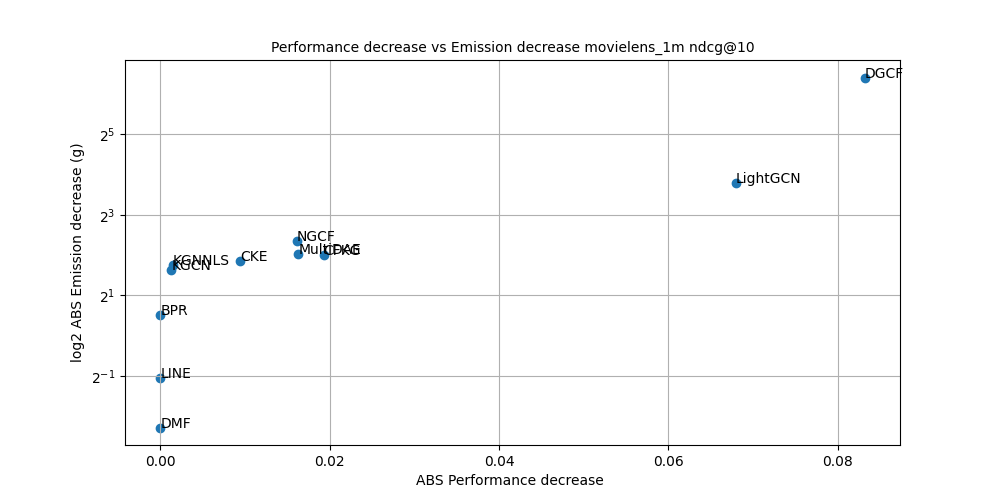
\includegraphics[scale=0.5]{images/decrement_ndcg@10_movielens_1m_30_5.png}
    \caption{Decremento di ndcg@10}
\end{figure}

\begin{figure}[H]
    \centering
    \includegraphics[scale=0.5]{images/decrement_recall@10_movielens_1m_30_5.png}
    \caption{Decremento di recall@10}
\end{figure}
\noindent Rispetto allo scorso esperimento, KGNNLS escluso, tutti i modelli hanno avuto un comportamento pressochè simile all'esperimento precedente emettendo leggermente di più. Dunque la combinazione di parametri 40 e 5 si è rivelata migliore di 30 e 5

\subsubsection{Terzo esperimento}
Il terzo esperimento è stato effettuato con una soglia di tolleranza pari a 40 e un numero di epoche consecutive pari a 6



\begin{table}[H]
    \centering
    \footnotesize
    \setlength\tabcolsep{0pt}
    \begin{tabularx}{\textwidth}{|X|X|}
        \hline
        \textbf{Criterio classico} & \textbf{Criterio modificato} \\
        \hline
        \includegraphics[width=\linewidth, trim=0 0 0 0]{images/emissions_movielens_1m_40_6_earlyClassic.png} &
        \includegraphics[width=\linewidth, trim=0 0 0 0]{images/emissions_movielens_1m_40_6_earlyModified.png} \\
        \hline
    \end{tabularx}
    \caption{Emissioni con criterio classico e modificato}
    \label{tab:emissions_info}
\end{table}



\begin{table}[H]
    \centering
    \resizebox{\textwidth}{!}{
    \begin{tabular}{|c|c|c|c|}
        \hline
        \textbf{Modello} & \textbf{Emissioni criterio classico (g)} & \textbf{Emissioni criterio nuovo (g)} & \textbf{\% riduzione emissioni}\\
        \hline
        BPR & 3.9484 & 2.483 & 37.1154 \\ \hline
        CKFG & 5.881 & 1.8037 & 69.3305 \\ \hline
        CKE & 5.6839 & 2.0806 & 63.3944 \\ \hline
        DMF & 2.2927 & 2.9977 & 12.869 \\ \hline
        KGCN & 6.8754 & 3.9708 & 42.2461 \\ \hline
        KGNNLS & 7.763 & 1.8709 & 75.8996 \\ \hline
        LINE & 1.9129 & 1.396 & 27.0205 \\ \hline
        MultiDAE & 8.0303 & 3.048 & 62.044 \\ \hline
        LightGCN & 15.626 & 1.7426 & 88.8482 \\ \hline
        NGCF & 7.7582 & 2.821 & 63.6387 \\ \hline
        DGCF & 94.903 & 11.8866 & 87.475 \\ \hline

    \end{tabular}
    }
    \caption{Confronto delle emissioni}
\end{table}

\noindent Rispetto al primo esperimento la percentuale di riduzioni delle emissioni in generale è diminuita. Rispetto al secondo esperimento, invece, la percentuale di riduzione delle emissioni è, in generale, leggermente aumentata (cioè ci sono state più emissioni).


\begin{figure}[H]
    \centering
    \includegraphics[width=\linewidth, trim=0 0 0 0]{images/recall@10_movielens_1m_40_6_comparison.png}
    \caption{Confronto score recall@10}
    
\end{figure}

\begin{figure}[H]
    \centering
    \includegraphics[width=\linewidth, trim=0 0 0 0]{images/ndcg@10_movielens_1m_40_6_comparison.png}
    \caption{Confronto score ndcg@10}
    
\end{figure}

\begin{figure}[H]
    \centering
    \includegraphics[width=\linewidth, trim=0 0 0 0]{images/giniindex@10_movielens_1m_40_6_comparison.png}
    \caption{Confronto score giniindex@10}
\end{figure}

\begin{figure}[H]
    \centering
    \includegraphics[width=\linewidth, trim=0 0 0 0]{images/averagepopularity@10_movielens_1m_40_6_comparison.png}
    \caption{Confronto score averagepopularity@10}
\end{figure}


\begin{table}[H]
    \centering
    \resizebox{\textwidth}{!}{
        \begin{tabular}{|c|c|c|c|c|}
    \hline
    \textbf{Modello} & \textbf{Metrica} & \textbf{Score criterio classico} & \textbf{Score criterio nuovo} & \textbf{\% riduzione score}\\
    \hline
    BPR & recall@10 & 0.1635 & 0.1635 & 0.0 \\ \hline
    CFKG & recall@10 & 0.1526 & 0.1301 & 14.7444 \\ \hline
    CKE & recall@10 & 0.1593 & 0.1517 & 4.7709 \\ \hline
    DMF & recall@10 & 0.1432 & 0.1432 & 0.0 \\ \hline
    KGCN & recall@10 & 0.1422 & 0.1422 & 0.0 \\ \hline
    KGNNLS & recall@10 & 0.1421 & 0.1232 & 13.3005 \\ \hline
    LINE & recall@10 & 0.1451 & 0.1451 & 0.0 \\ \hline
    MultiDAE & recall@10 & 0.1799 & 0.1531 & 14.8972 \\ \hline
    LightGCN & recall@10 & 0.173 & 0.1126 & 34.9133 \\ \hline
    NGCF & recall@10 & 0.1586 & 0.1438 & 9.3317 \\ \hline
    DGCF & recall@10 & 0.1656 & 0.108 & 34.7826 \\ \hline
    BPR & ndcg@10 & 0.2554 & 0.2554 & 0.0 \\ \hline
    CFKG & ndcg@10 & 0.2402 & 0.2209 & 8.035 \\ \hline
    CKE & ndcg@10 & 0.2534 & 0.2482 & 2.0521 \\ \hline
    DMF & ndcg@10 & 0.2289 & 0.2289 & 0.0 \\ \hline
    KGCN & ndcg@10 & 0.232 & 0.2328 & -0.3448 \\ \hline
    KGNNLS & ndcg@10 & 0.2319 & 0.2115 & 8.7969 \\ \hline
    LINE & ndcg@10 & 0.2277 & 0.2277 & 0.0 \\ \hline
    MultiDAE & ndcg@10 & 0.2633 & 0.2372 & 9.9126 \\ \hline
    LightGCN & ndcg@10 & 0.2682 & 0.1955 & 27.1066 \\ \hline
    NGCF & ndcg@10 & 0.2539 & 0.2401 & 5.4352 \\ \hline
    DGCF & ndcg@10 & 0.2613 & 0.1857 & 28.9323 \\ \hline
    BPR & averagepopularity@10 & 1146.3572 & 1146.3572 & 0.0 \\ \hline
    CFKG & averagepopularity@10 & 1115.4498 & 1361.1447 & -22.0265 \\ \hline
    CKE & averagepopularity@10 & 1165.2413 & 1320.1912 & -13.2977 \\ \hline
    DMF & averagepopularity@10 & 1379.7292 & 1379.7292 & 0.0 \\ \hline
    KGCN & averagepopularity@10 & 1188.9582 & 1187.2098 & 0.1471 \\ \hline
    KGNNLS & averagepopularity@10 & 1188.8981 & 1401.0945 & -17.8482 \\ \hline
    LINE & averagepopularity@10 & 979.498 & 979.498 & 0.0 \\ \hline
    MultiDAE & averagepopularity@10 & 1137.4597 & 1297.2825 & -14.0509 \\ \hline
    LightGCN & averagepopularity@10 & 1088.741 & 1649.9548 & -51.547 \\ \hline
    NGCF & averagepopularity@10 & 1201.8831 & 1407.3654 & -17.0967 \\ \hline
    DGCF & averagepopularity@10 & 1172.6874 & 1760.7243 & -50.1444 \\ \hline
    BPR & giniindex@10 & 0.8839 & 0.8839 & 0.0 \\ \hline
    CFKG & giniindex@10 & 0.8822 & 0.9401 & -6.5631 \\ \hline
    CKE & giniindex@10 & 0.8894 & 0.9266 & -4.1826 \\ \hline
    DMF & giniindex@10 & 0.9443 & 0.9443 & 0.0 \\ \hline
    KGCN & giniindex@10 & 0.8992 & 0.8984 & 0.089 \\ \hline
    KGNNLS & giniindex@10 & 0.8992 & 0.945 & -5.0934 \\ \hline
    LINE & giniindex@10 & 0.8904 & 0.8904 & 0.0 \\ \hline
    MultiDAE & giniindex@10 & 0.875 & 0.9204 & -5.1886 \\ \hline
    LightGCN & giniindex@10 & 0.8759 & 0.9767 & -11.5082 \\ \hline
    NGCF & giniindex@10 & 0.9079 & 0.9481 & -4.4278 \\ \hline
    DGCF & giniindex@10 & 0.8992 & 0.982 & -9.2082 \\ \hline
\end{tabular}
    }
    \caption{Performance dei modelli su diverse metriche e dataset}
    \end{table}


\begin{figure}[H]
    \centering
    \includegraphics[scale=0.5]{images/decrement_averagepopularity@10_movielens_1m_40_6.png}
    \caption{Decremento di averagepopularity@10}
\end{figure}

\begin{figure}[H]
    \centering
    \includegraphics[scale=0.5]{images/decrement_giniindex@10_movielens_1m_40_6.png}
    \caption{Decremento di giniindex@10}
\end{figure}

\begin{figure}[H]
    \centering
    \includegraphics[scale=0.5]{images/decrement_ndcg@10_movielens_1m_40_6.png}
    \caption{Decremento di ndcg@10}
\end{figure}

\begin{figure}[H]
    \centering
    \includegraphics[scale=0.5]{images/decrement_recall@10_movielens_1m_40_6.png}
    \caption{Decremento di recall@10}
\end{figure}

\noindent Rispetto al primo esperimento la riduzione delle performance sono diminuite (cioè gli algoritmi hanno performato meglio). Anche rispetto al secondo esperimento (con alcune eccezzioni come KGNNLS) le performance sonoo più alte, anche se di poco.




\subsubsection{Quarto esperimento}
Il quarto esperimento è stato effettuato con una soglia di tolleranza pari a 30 e un numero di epoche consecutive pari a 6



\begin{table}[H]
    \centering
    \footnotesize
    \setlength\tabcolsep{0pt}
    \begin{tabularx}{\textwidth}{|X|X|}
        \hline
        \textbf{Criterio classico} & \textbf{Criterio modificato} \\
        \hline
        \includegraphics[width=\linewidth, trim=0 0 0 0]{images/emissions_movielens_1m_30_6_earlyClassic.png} &
        \includegraphics[width=\linewidth, trim=0 0 0 0]{images/emissions_movielens_1m_30_6_earlyModified.png} \\
        \hline
    \end{tabularx}
    \caption{Emissioni con criterio classico e modificato}
    \label{tab:emissions_info}
\end{table}



\begin{table}[H]
    \centering
    \resizebox{\textwidth}{!}{
    \begin{tabular}{|c|c|c|c|}
        \hline
        \textbf{Modello} & \textbf{Emissioni criterio classico (g)} & \textbf{Emissioni criterio nuovo (g)} & \textbf{\% riduzione emissioni}\\
        \hline
        BPR & 3.9484 & 3.1221 & 20.93 \\ \hline
        CFKG & 5.881 & 1.9202 & 67.35 \\ \hline
        CKE & 5.6839 & 2.078 & 63.44 \\ \hline
        DMF & 2.2927 & 1.9962 & 12.93 \\ \hline
        KGCN & 6.8754 & 3.9292 & 42.85 \\ \hline
        KGNNLS & 7.763 & 4.7984 & 38.19 \\ \hline
        LINE & 1.9129 & 1.3937 & 27.14 \\ \hline
        MultiDAE & 8.0303 & 3.7405 & 53.42 \\ \hline
        LightGCN & 15.626 & 2.1161 & 86.46 \\ \hline
        NGCF & 7.7582 & 2.885 & 62.81 \\ \hline
        DGCF & 94.903 & 12.0604 & 87.2918 \\ \hline

    \end{tabular}
    }
    \caption{Confronto delle emissioni}
\end{table}

\noindent Rispetto a tutti e tre gli esperimenti precedenti la percentuale di riduzioni delle emissioni in generale è diminuita, dunque gli algoritmi hanno emesso di più.


\begin{figure}[H]
    \centering
    \includegraphics[width=\linewidth, trim=0 0 0 0]{images/recall@10_movielens_1m_30_6_comparison.png}
    \caption{Confronto score recall@10}
    
\end{figure}

\begin{figure}[H]
    \centering
    \includegraphics[width=\linewidth, trim=0 0 0 0]{images/ndcg@10_movielens_1m_30_6_comparison.png}
    \caption{Confronto score ndcg@10}
    
\end{figure}

\begin{figure}[H]
    \centering
    \includegraphics[width=\linewidth, trim=0 0 0 0]{images/giniindex@10_movielens_1m_30_6_comparison.png}
    \caption{Confronto score giniindex@10}
\end{figure}

\begin{figure}[H]
    \centering
    \includegraphics[width=\linewidth, trim=0 0 0 0]{images/averagepopularity@10_movielens_1m_30_6_comparison.png}
    \caption{Confronto score averagepopularity@10}
\end{figure}


\begin{table}[H]
    \centering
    \resizebox{\textwidth}{!}{
        \begin{tabular}{|c|c|c|c|c|}
    \hline
    \textbf{Modello} & \textbf{Metrica} & \textbf{Score criterio classico} & \textbf{Score criterio nuovo} & \textbf{\% riduzione score}\\
    \hline
    BPR & recall@10 & 0.1635 & 0.1635 & 0.0 \\ \hline
    CFKG & recall@10 & 0.1526 & 0.1344 & 11.9266 \\ \hline
    CKE & recall@10 & 0.1593 & 0.1517 & 4.7709 \\ \hline
    DMF & recall@10 & 0.1432 & 0.1432 & 0.0 \\ \hline
    KGCN & recall@10 & 0.1422 & 0.1422 & 0.0 \\ \hline
    KGNNLS & recall@10 & 0.1421 & 0.1421 & 0.0 \\ \hline
    LINE & recall@10 & 0.1451 & 0.1451 & 0.0 \\ \hline
    MultiDAE & recall@10 & 0.1799 & 0.1624 & 9.7276 \\ \hline
    LightGCN & recall@10 & 0.173 & 0.1204 & 30.4046 \\ \hline
    NGCF & recall@10 & 0.1586 & 0.1438 & 9.3317 \\ \hline
    DGCF & recall@10 & 0.1656 & 0.108 & 34.7826 \\ \hline
    BPR & ndcg@10 & 0.2554 & 0.2554 & 0.0 \\ \hline
    CFKG & ndcg@10 & 0.2402 & 0.2245 & 6.5362 \\ \hline
    CKE & ndcg@10 & 0.2534 & 0.2482 & 2.0521 \\ \hline
    DMF & ndcg@10 & 0.2289 & 0.2289 & 0.0 \\ \hline
    KGCN & ndcg@10 & 0.232 & 0.2328 & -0.3448 \\ \hline
    KGNNLS & ndcg@10 & 0.2319 & 0.2327 & -0.345 \\ \hline
    LINE & ndcg@10 & 0.2277 & 0.2277 & 0.0 \\ \hline
    MultiDAE & ndcg@10 & 0.2633 & 0.2463 & 6.4565 \\ \hline
    LightGCN & ndcg@10 & 0.2682 & 0.2064 & 23.0425 \\ \hline
    NGCF & ndcg@10 & 0.2539 & 0.2401 & 5.4352 \\ \hline
    DGCF & ndcg@10 & 0.2613 & 0.1857 & 28.9323 \\ \hline
    BPR & averagepopularity@10 & 1146.3572 & 1146.3572 & 0.0 \\ \hline
    CFKG & averagepopularity@10 & 1115.4498 & 1338.642 & -20.0092 \\ \hline
    CKE & averagepopularity@10 & 1165.2413 & 1320.1912 & -13.2977 \\ \hline
    DMF & averagepopularity@10 & 1379.7292 & 1379.7292 & 0.0 \\ \hline
    KGCN & averagepopularity@10 & 1188.9582 & 1187.2098 & 0.1471 \\ \hline
    KGNNLS & averagepopularity@10 & 1188.8981 & 1187.2158 & 0.1415 \\ \hline
    LINE & averagepopularity@10 & 979.498 & 979.498 & 0.0 \\ \hline
    MultiDAE & averagepopularity@10 & 1137.4597 & 1238.6498 & -8.8961 \\ \hline
    LightGCN & averagepopularity@10 & 1088.741 & 1585.7381 & -45.6488 \\ \hline
    NGCF & averagepopularity@10 & 1201.8831 & 1407.3654 & -17.0967 \\ \hline
    DGCF & averagepopularity@10 & 1172.6874 & 1760.6621 & -50.1391 \\ \hline
    BPR & giniindex@10 & 0.8839 & 0.8839 & 0.0 \\ \hline
    CFKG & giniindex@10 & 0.8822 & 0.9367 & -6.1777 \\ \hline
    CKE & giniindex@10 & 0.8894 & 0.9266 & -4.1826 \\ \hline
    DMF & giniindex@10 & 0.9443 & 0.9443 & 0.0 \\ \hline
    KGCN & giniindex@10 & 0.8992 & 0.8984 & 0.089 \\ \hline
    KGNNLS & giniindex@10 & 0.8992 & 0.8983 & 0.1001 \\ \hline
    LINE & giniindex@10 & 0.8904 & 0.8904 & 0.0 \\ \hline
    MultiDAE & giniindex@10 & 0.875 & 0.9054 & -3.4743 \\ \hline
    LightGCN & giniindex@10 & 0.8759 & 0.9709 & -10.846 \\ \hline
    NGCF & giniindex@10 & 0.9079 & 0.9481 & -4.4278 \\ \hline
    DGCF & giniindex@10 & 0.8992 & 0.982 & -9.2082 \\ \hline
\end{tabular}
    }
    \caption{Performance dei modelli su diverse metriche e dataset}
    \end{table}


\begin{figure}[H]
    \centering
    \includegraphics[scale=0.5]{images/decrement_averagepopularity@10_movielens_1m_30_6.png}
    \caption{Decremento di averagepopularity@10}
\end{figure}

\begin{figure}[H]
    \centering
    \includegraphics[scale=0.5]{images/decrement_giniindex@10_movielens_1m_30_6.png}
    \caption{Decremento di giniindex@10}
\end{figure}

\begin{figure}[H]
    \centering
    \includegraphics[scale=0.5]{images/decrement_ndcg@10_movielens_1m_30_6.png}
    \caption{Decremento di ndcg@10}
\end{figure}

\begin{figure}[H]
    \centering
    \includegraphics[scale=0.5]{images/decrement_recall@10_movielens_1m_30_6.png}
    \caption{Decremento di recall@10}
\end{figure}

\noindent Rispetto ai 3 esperimenti la percentuale di riduzione delle performance è diminuita. Per ora dunque questo è l'esperimento che ha emesso di più e performato.

